%
% Unless otherwise indicated, the copyright in this material is 
% owned by Joerg Evermann. This material is licensed to you under the 
% Creative Commons by-attribution non-commercial license (CC BY-NC 4.0)}
%

\section*{Sources and Further Reading}

The material in this chapter is based on the following sources.

\begin{tcolorbox}[colback=alert]
Tom White (2012) \emph{Hadoop -- The Definitive Guide}. 3rd edition. O'Reilly Media. Sebastopol, California, US.
\end{tcolorbox}

This book introduces in great detail the main concepts of Apache Hadoop and provides step-by-step introduction to setting up a Hadoop cluster, using the Map-Reduce API, submitting and managing jobs. The book also provides a chapter on related projects, such as Hive and Pig. It was written for Hadoop 2.3, which introduced the Map-Reduce 2.0 API and YARN. While older, it can still serve as a comprehensive reference also to more recent Hadoop versions.

\begin{tcolorbox}[colback=alert]
Hrishikesh V. Karambelkar (2018) \emph{Apache Hadoop 3 Quick Start Guide}. Packt Publishing. Birmingham, UK.
\end{tcolorbox}

This quick start guide is more recent and written for Hadoop 3.0. It provides only a brief overview of the Hadoop system, focusing on cluster installation, configuration, and management, rather than Map-Reduce or data management.

\begin{tcolorbox}[colback=alert]
Bill Chambers and Matei Zaharia (2018) \emph{Spark -- The Definitive Guide}. O'Reilly Media. Sebastopol, California, US.
\end{tcolorbox}

This is a very comprehensive book, written for Spark 2.0. Matei Zaharia is the original designer and lead developer of the Spark project. The book covers all aspects of Spark. All examples are provided both in Scala and in Python. While a little older at this point, it is very instructive and easy to follow with many practical points of how to get the most out of Spark.

\begin{tcolorbox}[colback=alert]
Jules Damji et al. (2020) \emph{Learning Spark -- Lightning-Fast Data Analytics}. 2nd edition. O'Reilly Media. Sebastopol, California, US.
\end{tcolorbox}

This book, while not quite as comprehensive as the one by Chambers \& Zaharia, is newer and targets Spark 3.0. It also covers all aspects of Spark, from installation and configuration, to programming the SQL, streaming, and machine learning components of Spark. The book provides most examples in both Scala and Python.

\begin{tcolorbox}[colback=alert]
\subsubsection*{Resources}
Complete implementations of all examples in this chapter are available in the following GitHub repos.\\

For the Hadoop MapReduce examples:

\url{https://github.com/jevermann/busi4720-hadoop} \\

The project can be cloned from this URL:

\url{https://github.com/jevermann/busi4720-hadoop.git} \\

For the Spark examples:

\url{https://github.com/jevermann/busi4720-pyspark} \\

The project can be cloned from this URL:

\url{https://github.com/jevermann/busi4720-pyspark.git} \\
\end{tcolorbox}

\section{Introduction}

Big data analytics refers to the process of examining large and varied data sets -- \emph{big data} -- to uncover hidden patterns, unknown correlations, market trends, customer preferences, and other useful information that can help organizations make better-informed business decisions. Driven by specialized analytics systems and software, big data analytics can lead to more effective marketing, new revenue opportunities, better customer service, improved operational efficiency, competitive advantages over rival organizations, and other business benefits.

The term ''big data'' is typically associated with three key concepts: data volume, data variety, and data velocity. Together, these three Vs define the challenges and opportunities that organizations face when managing and analyzing massive data sets. The emergence of the fourth and fifth Vs, data veracity and data value, reflect the increasing need to ensure the reliability of data and the importance of deriving meaningful insight from it.

\paragraph*{Volume} represents the quantity of data that is generated and stored. It is one of the primary characteristics of big data. Organizations collect data from a variety of sources, including business transactions, smart (IoT, Internet-of-Things) devices, industrial equipment, videos, social media, and more. As data volume increases, the value and potential insights also increase, but it requires more effective data management and processing technologies. The challenge lies not only in the storage but also in dynamically scaling resources to process this vast amount of data efficiently.

\paragraph*{Variety} refers to the different types of data that are available, both structured and unstructured. Traditional data types were structured and fit neatly in a relational database. However, with the advent of big data, data comes in new unstructured forms such as text, images, videos, and social media posts. The variety in data types frequently requires additional preprocessing to derive meaning and supports analytics that can lead to enhanced business insights.

\paragraph*{Velocity} is the speed at which the data is generated, collected, and processed. High velocity of big data comes from connected sensors, smart devices, web page streaming, and other live feeds. Managing the velocity of data entails not only processing these streams effectively but also ensuring that data analysis and decision making are conducted in a timely manner.

\paragraph*{Veracity} refers to the accuracy of data. Big data veracity deals with the assurance of quality and accuracy of data considering its volume, variety, and velocity. This characteristic is crucial as it affects every decision made based on big data. Poor data quality can lead to incorrect conclusions. Therefore, organizations must invest in analytic processes that validate and cleanse data to ensure accuracy and usefulness.

\paragraph*{Value} value is about turning big data into business value. This is the most important V of all, as it determines whether the data collected and analyzed are of any use to the organization. The main challenge is to sift through vast lakes of data and find what is relevant and can be turned into actionable insights that can lead to cost reductions, improved efficiency, or new revenue opportunities.

An example of a big data use case is the Conseil Europeenne pour la Recherche Nucleair (CERN). CERN is the world's largest physicas laboratory, an international cooperation that researches high-energy particle physics located in Switzerland and France. When physics experiments are running, the CERN data center processes about one petabye (one million gigabyte) of data per day\footnote{\url{https://www.home.cern/science/computing/storage}, last accessed June 10, 2024}. Preparations are under way for new physics experiments that require storage and analysis of 600 petabytes of data. Table~\ref{tab:cern} provides an overview over the CERN data centre infrastructure to manage this volume and this velocity of data. 

Figure~\ref{fig:cerndata} shows images of the CERN data centre infrastructure. Racks are filled with multiple computer servers, each with their own attached data storage, and multiple racks are lined up in rows. Computers are networked, first within a rack, then between racks, and the data center is connected to the larger internet. Network connections are fastest between computers within the same rack, then between computers in different racks, and are slowest across the internet. 

Clearly, the volume of data being stored, and the velocity with which it is generated requires analytics techniques and software tools that go beyond those of single-machine or desktop solutions examined so far, like R, Numpy or Pandas, and that are suitable to efficiently use infrastructure like the one shown in Figure~\ref{fig:cerndata}. The following sections introduce big data analytics, or data analytics at industrial scales. 

\begin{table}
\centering

\renewcommand{\arraystretch}{1.25}
\begin{tabular}{l r l} \hline
Servers & $\approx 12000$ \\
CPU Cores & $\approx 350000$ \\
Disks & $\approx 220000$ \\
Total Disk Space & $\approx 950000$ & TB \\ 
DB Transactions per second & $\approx 20000$ \\ 
File Transfer Throughput & $\approx 100$ & Gb/s\\  \hline
\end{tabular}
\caption[Data management infrastructure at CERN]{Data management infrastructure at CERN\footnotemark}
\label{tab:cern}
\end{table}
\footnotetext{\url{https://www.home.cern/science/computing/data-centre}, last accessed June 10, 2024}

\begin{figure}
\centering

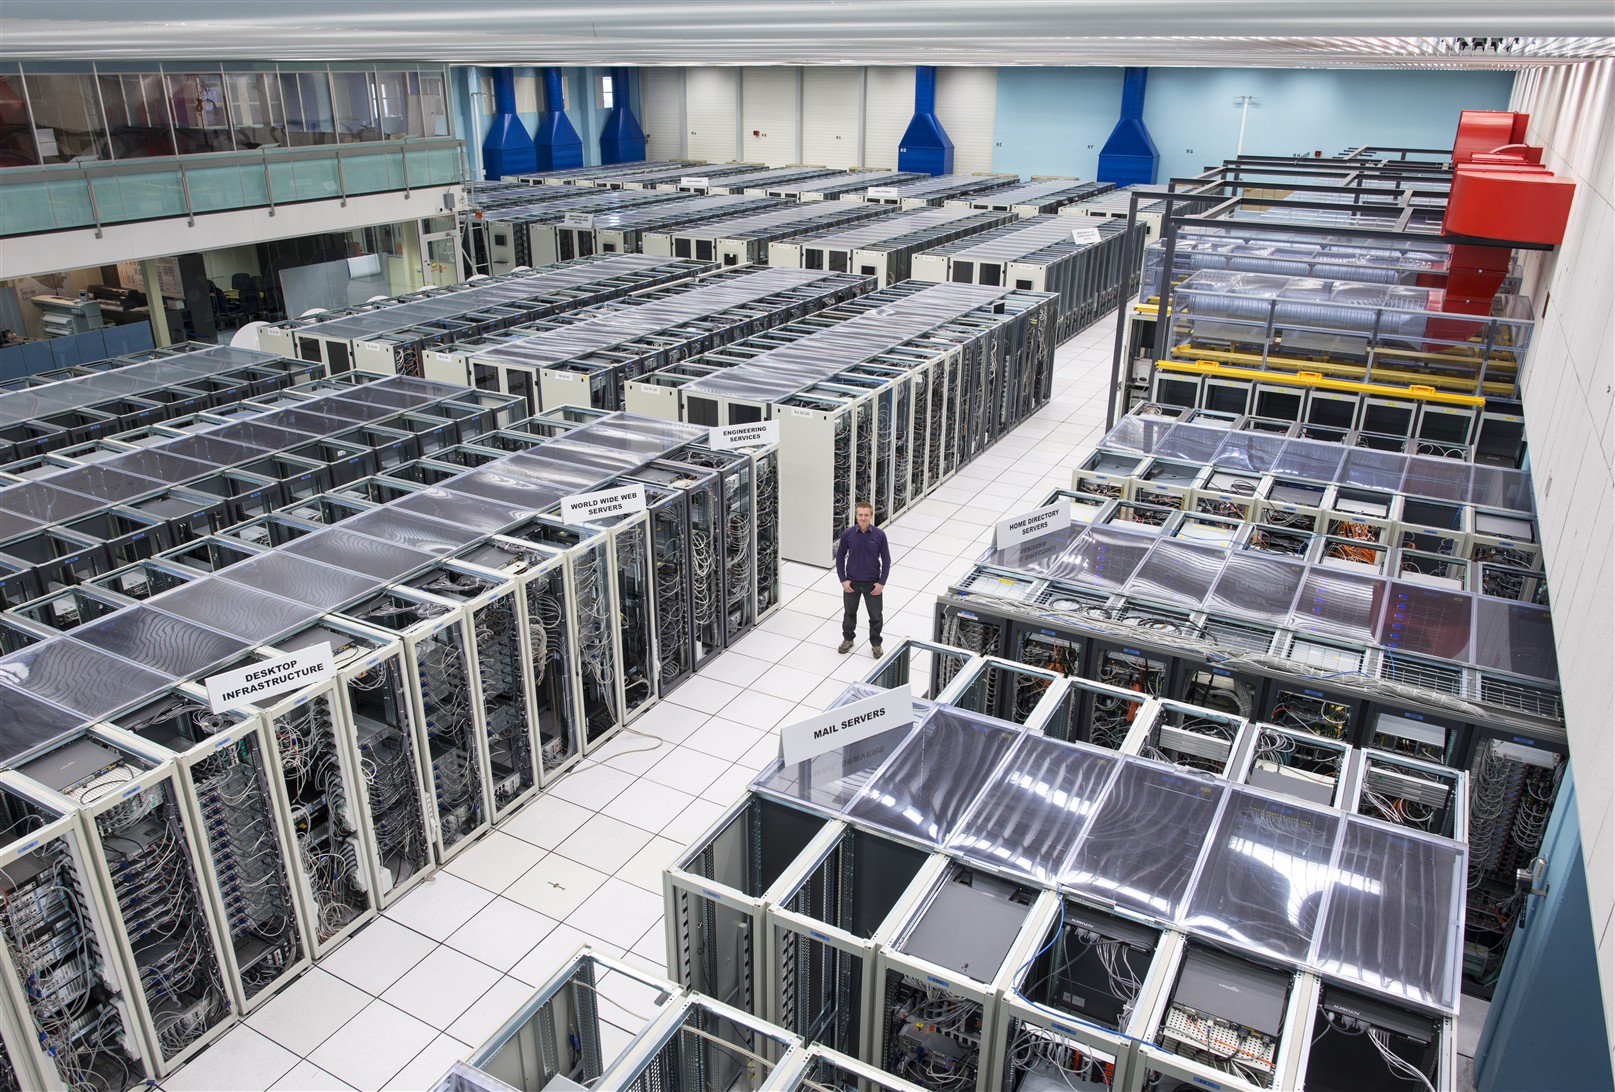
\includegraphics[width=.45\textwidth]{cern1.jpg} \hfill
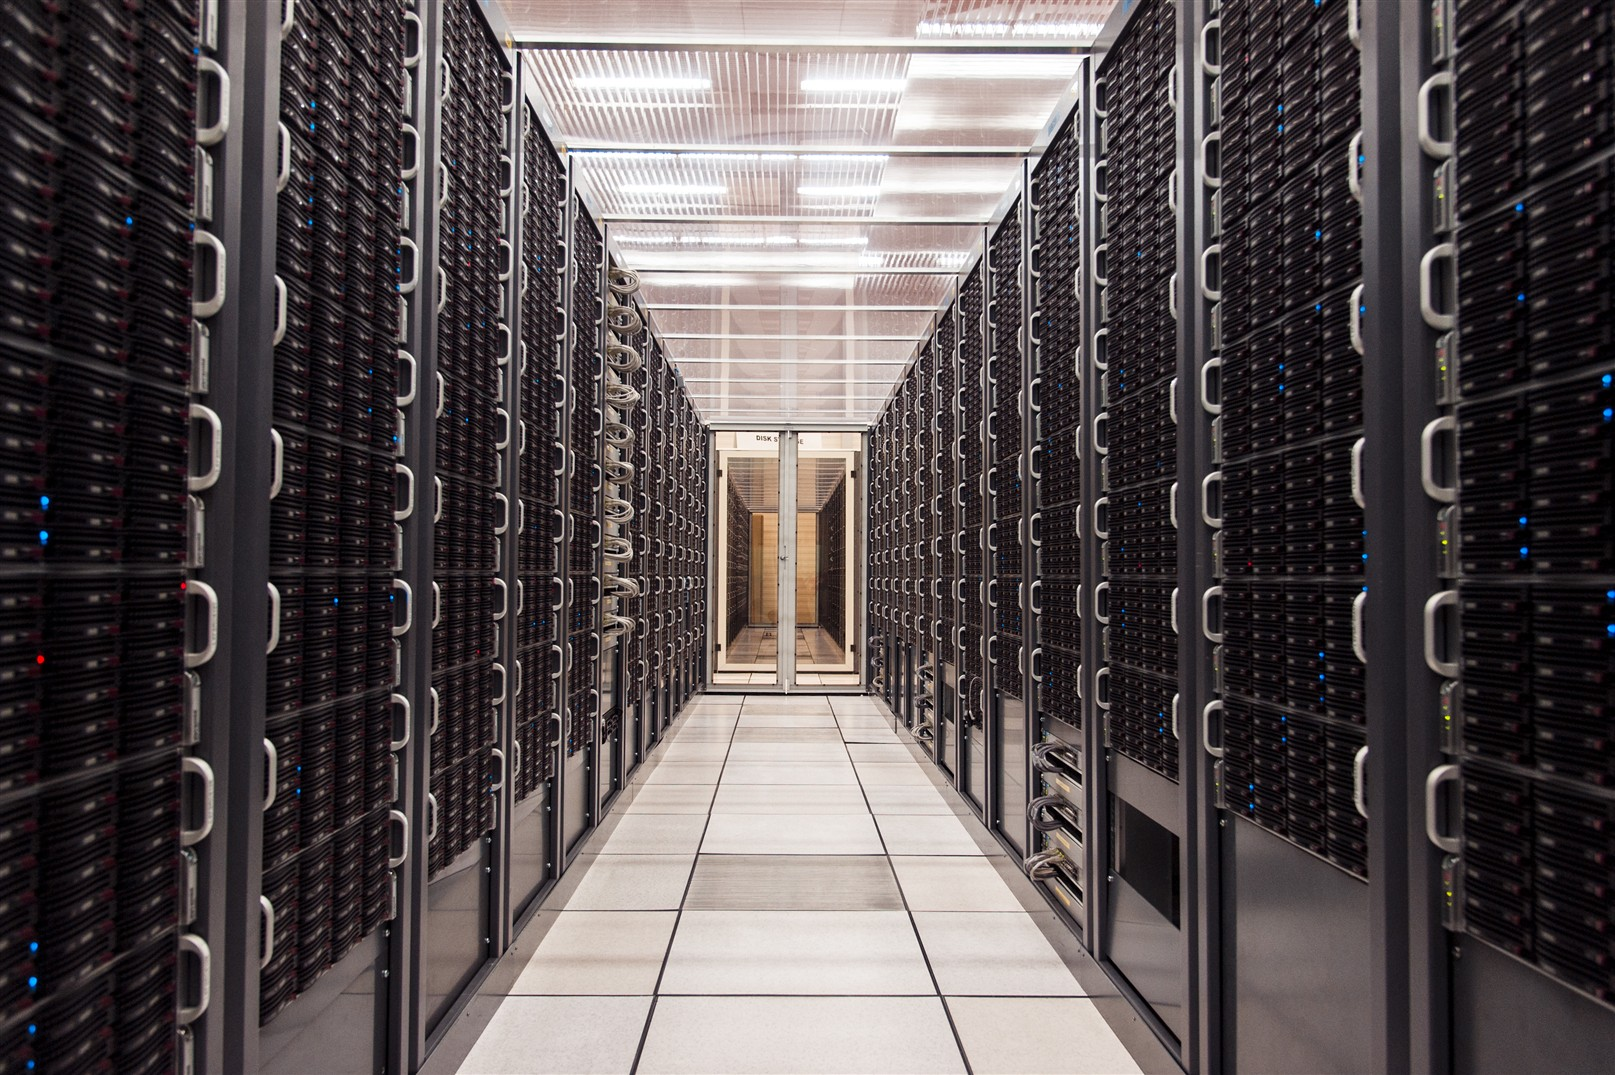
\includegraphics[width=.45\textwidth]{cern2.jpg} \\

\scriptsize Source: CERN.org with \href{https://copyright.web.cern.ch/}{permission} \normalsize
\caption{CERN data centre images}
\label{fig:cerndata}
\end{figure}

\FloatBarrier

\section{Hadoop}

\begin{wrapfigure}{l}{.33\textwidth}
\begin{center}

\includegraphics[width=.33\textwidth]{Apache_Hadoop.png}
\scriptsize \url{https://commons.wikimedia.org/wiki/File:Apache_Hadoop.png}
\end{center}
\end{wrapfigure}

Apache Hadoop is an open-source system for distributed data storage and distribute computation on data. Initially released in 2006, it is maintained by the Apache Foundation. It was originally inspired by the Google File System (GFS) that Google used to manage its web search data\footnote{Ghemawat, S., Gobioff, H., \& Leung, S. T. (2003, October). The Google file system. In Proceedings of the nineteenth ACM symposium on Operating systems principles (pp. 29-43).}, and the Google MapReduce technique for computations on distributed data\footnote{Dean, J., \& Ghemawat, S. (2008). MapReduce: simplified data processing on large clusters. Communications of the ACM, 51(1), 107-113.}. Early successful uses cases at Yahoo in 2009 and at Facebook in 2012 drove industry adoption and further research interest. Hadoop relies on a distributed file system called HDFS (''Hadoop Distributed File System'') that distributes data storage across a cluster of computers. In contrast to other solutions at the time, the clusters did not require specialized hardware or software, which made the system very attractive to organizations. 

The main principle of data procesing with Hadoop is \emph{data locality}: Instead of moving data across network connections to the computer where computation takes place, which is expensive and slow, computation is moved to where the data is stored. In other words, data is processed where it is stored, in a distributed fashion.

The benefits that make Hadoop attractive are its reliability, scalability, cost effectiveness and cloud support. 

\paragraph*{Reliability}

Hadoop is highly reliable. It stores multiple copies of data across different computer nodes in a network, ensuring that the system can tolerate the failure of any network node without data loss. This redundancy provides fault tolerance, as data is automatically re-replicated from the remaining copies when a network node fails, allowing data processing to continue uninterrupted.

\paragraph*{Scalability}

Scalability is one of Hadoop's core strengths. It can store and distribute very large data sets across hundreds to thousands of inexpensive servers that operate in parallel. This distributed computing model allows businesses to scale up or down efficiently without downtime. As more servers are added, Hadoop continues to increase its storage capacity, processing power, and throughput performance proportionally.

\paragraph*{Cost Effectiveness}

Hadoop is cost-effective. As open-source software, combined with the use of commodity hardware, it significantly reduces the cost of a system capable of storing and processing enormous amounts of data. The cost savings are not just in terms of hardware but also in scalability. Businesses can start with what they need and increase their system size as they grow while maintaining a low cost per terabyte. Hadoop 3 provides support clusters with more than 10,000 computers.

\paragraph*{Cloud Support}

Finally, Hadoop supports cloud-based services, which allows businesses to deploy Hadoop clusters in cloud environments. This capability means that organizations can benefit from cloud computing features, such as massive scalability, on-demand resource allocation, and utility-based cost structures. Most major cloud vendors, such as Amazon Web Services (AWS), Google Cloud Platform (GCP), and Microsoft Azure offer Hadoop or equivalent services to their customers.

Hadoop consists of three main components. HDFS is the storage layer of Hadoop. It is a distributed file system designed to run on commodity hardware. MapReduce is a programming model and implementation for processing large data sets with a parallel, distributed algorithm, and YARN is the resource management layer of Hadoop. 

\subsection{HDFS}

HDFS is designed and optimized for storing very large datasets, raning from a few gigabytes to hundreds of terabytes in size. HDFS is designed based on a number of fundamental principles: Data in HDFS is written and read linearly, and must processed one item at a time. For analytics applications, this means that applications cannot read arbitrary data or move back and forth in the data set. Once a file is written and closed, it cannot be changed, other than by appending data or truncating the file. This means that existing data in the file cannot be overwritten. If necessary, a new file must be created. HDFS is built around the idea of streaming data access, that means it emphasizes high throughput over low latency. In other words, accessing the same amount of data from one continuous file is much faster than accessing the same amount of data from multiple separate files. 

\begin{figure}
\centering

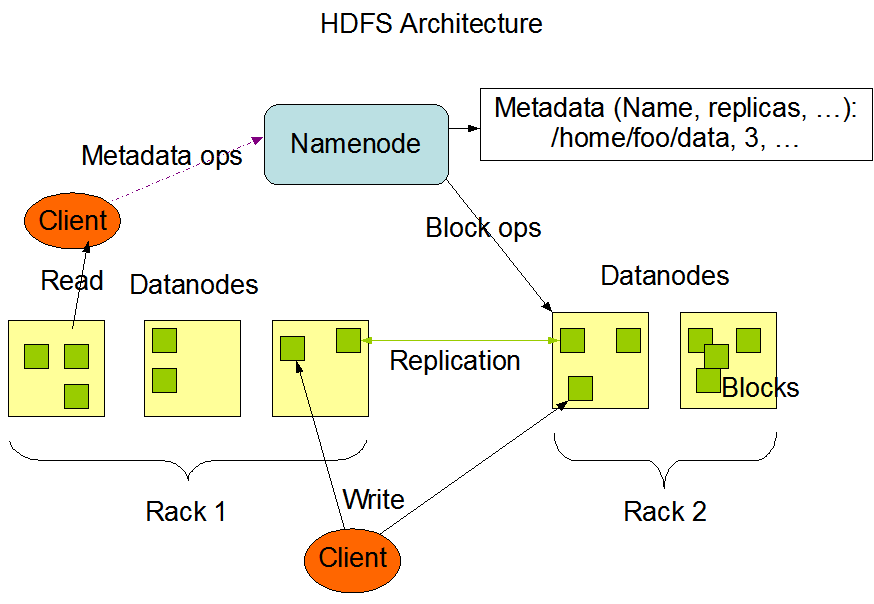
\includegraphics[width=.75\textwidth]{hdfsarchitecture.png} \\

\scriptsize Source: Apache Foundation (\url{https://hadoop.apache.org/docs/})
\caption{HDFS architecture}
\label{fig:hdfsarchitecture}
\end{figure}

Figure~\ref{fig:hdfsarchitecture} shows the architecture of HDFS. An HDFS cluster consists of a single Namenode (optionally a secondary/backup NameNode for fault tolerance), which is a server that runs software to manage the file system namespace and regulates access to files by client applications. The Namenode keeps the directory of all files in the file system, and tracks where on the cluster the file data is kept. The Namenode does not store actual data. Instead, it stores metadata, such as the location of blocks stored on the Datanodes, access permissions, and other information. It provides file operations such as opening, closing, renaming of files. Client applications communicate with the Namenode whenever they wish to locate a file, or when they want to add/copy/move/delete/\ldots a file. The Namenode responds to the requests by returning a list of relevant DataNode servers where the data lives.

Datanodes manage the storage attached to the computers they run on and serve read/write requests from the file system's client applications. HDFS splits large files into blocks (the default block size is 128MB) and distributes them across nodes in a cluster to enable high throughput access to data. The file system also replicates each data block multiple times (by default 3 times) across different nodes to ensure reliability and fault tolerance. Datanodes store and retrieve blocks when they are told to (by client applications or the NameNode), and they report back to the Namenode periodically with a list of blocks that they are storing.

Working with HDFS is very similar to working with the local file system on a desktop machine. In other words, the cluster is transparent. HDFS file commands are based on the standard Unix/Linux file commands to manipulate files and directories. The set of basic HDFS commands is shown in Table~\ref{tab:hdfscommands}. Because HDFS emphasizes throughput over latency, file operations that only involve small amounts of data, tend to be much slower than on a local file system.

In addition to the command line interface, the Hadoop Namenode also typically provides web-based access. For example, the Namenode overview can be accessed at \url{http://localhost:9870} (substitute another URL or host name if necessary) and will show the status of the datanodes in the cluster as well. This also allows browsing the file system and performing file operations, including uploading and downloading of files from and to the local filesystem through the HDFS explorer at \url{http://localhost:9870/explorer.html#/} (substitute another host name if necessary). Figure~\ref{fig:hdfswebaccess} shows a screenshot of the HDFS explorer.

\begin{figure}
\centering
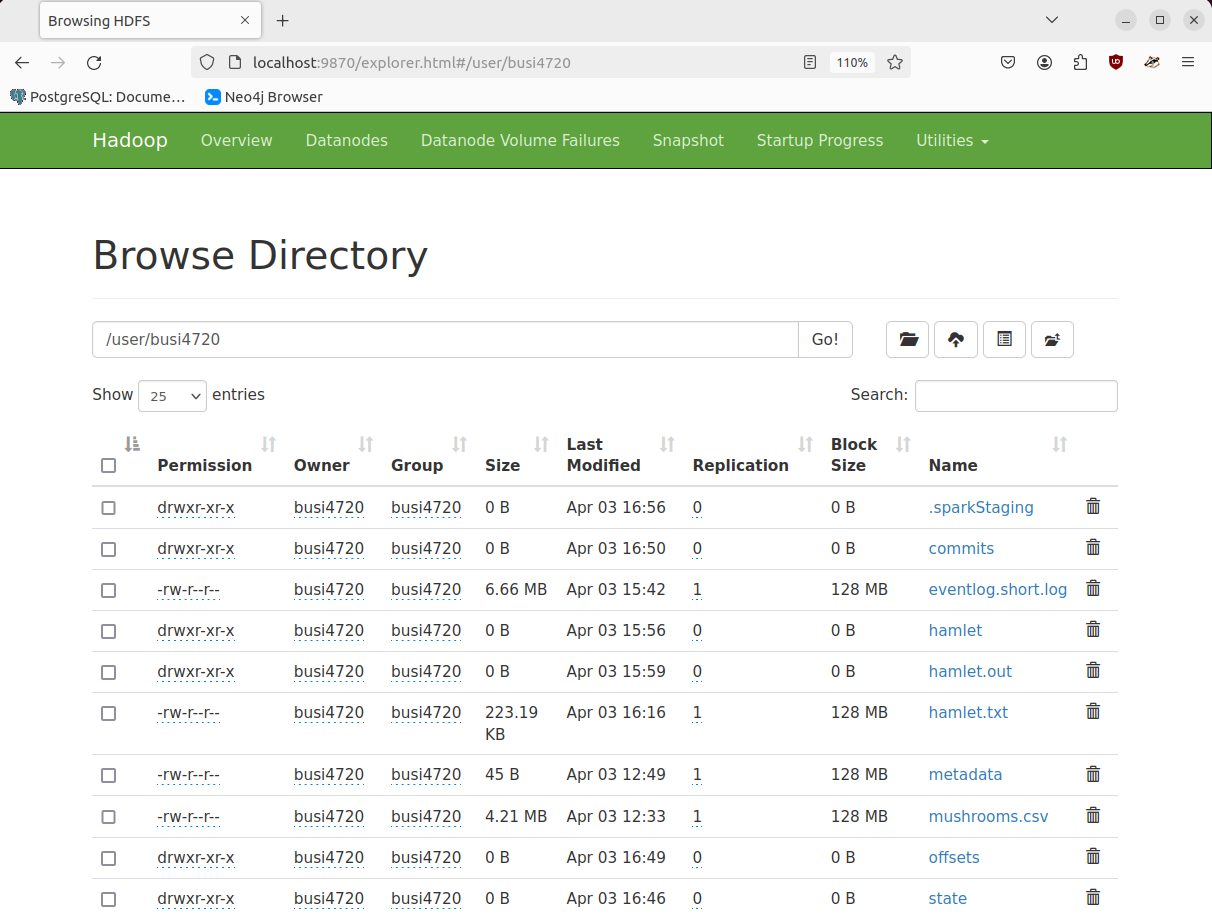
\includegraphics[width=.75\textwidth]{hdfs_web_access.png}
\caption{HDFS Explorer}
\label{fig:hdfswebaccess}
\end{figure}

\begin{table}
\centering

\renewcommand{\arraystretch}{1.25}
\small
\begin{tabular}{l|l} \hline
\texttt{hdfs dfs -cat} & Print a file to standard output \\
\texttt{hdfs dfs -cp} & Copy a file or directory\\
\texttt{hdfs dfs -df} & Display free space \\
\texttt{hdfs dfs -du} & Display disk usage \\
\texttt{hdfs dfs -get} & Copy files to the local file system \\
\texttt{hdfs dfs -head} & Print the first kilobyte of a file \\
\texttt{hdfs dfs -ls} & List files and directories \\
\texttt{hdfs dfs -mkdir} & Make a directory \\
\texttt{hdfs dfs -mv} & Move a file or directory \\
\texttt{hdfs dfs -put} & Copy files from the local file system \\
\texttt{hdfs dfs -rm} & Remove files or directories \\
\texttt{hdfs dfs -rmdir} & Removes a directory \\
\texttt{hdfs dfs -tail} & Print the last kilobyt of a file \\
\texttt{hdfs dfs -concat} & Concatenate existing files into a target file \\ \hline
\end{tabular}
\caption{Basic HDFS file system commands}
\label{tab:hdfscommands}
\end{table}

The following exercises illustrate the use of the HDFS. Use the \texttt{hdfs dfs} command to insteract with the distributed file system. The commands are similar to the regular Linux commands to interact with files.

One a single-machine cluster, the Hadoop Namenode, Datanode, and the YARN software applications are all installed on the same computer. Start the Hadoop cluster Namenode, Datanode, and YARN service as follows:

\begin{bashcode}
sudo systemctl start hadoop.service
\end{bashcode}

Download an event log file to your local file system and then put the event log onto the Hadoop Distributed File System:

\begin{samepage}
\begin{bashcode}
wget https://evermann.ca/busi4720/eventlog.short.log
hdfs dfs -put eventlog.short.log
\end{bashcode}
\end{samepage}

Display the start and end of the from the HDFS:
\begin{samepage}
\begin{bashcode}
hdfs dfs -head eventlog.short.log
hdfs dfs -tail eventlog.short.log
\end{bashcode}
\end{samepage}

Show disk usage and disk free space:
\begin{samepage}
\begin{bashcode}
hdfs dfs -du
hdfs dfs -df
\end{bashcode}
\end{samepage}

Copy the event log:
\begin{bashcode}
hdfs dfs -cp eventlog.short.log eventlog.copy.log
\end{bashcode}

List all files:
\begin{bashcode}
hdfs dfs -ls
\end{bashcode}


\begin{tcolorbox}[colback=code]
\subsubsection*{Hands-On Exercise} 

\paragraph*{Exercise 1: Accessing HDFS}

\begin{enumerate}
  \item View the list of files on the HDFS file system.
  \item Create a new directory in the HDFS named ''testdir''.
  \item Verify that 'testdir' has been created by listing all files.
\end{enumerate}

\paragraph*{Exercise 2: Manipulating Files in HDFS}

\begin{enumerate}
  \item Use a text editor to create a text file called ''example.txt'' on your local file system and write ''Hello HDFS'' into it.
  \item Copy ''example.txt'' from your local file system to the directory ''testdir'' in the HDFS.
  \item Read the contents of the file from the HDFS.
  \item Delete ''example.txt'' from the HDFS.
\end{enumerate}

\paragraph*{Exercise 3: Understanding HDFS Block Size}

\begin{enumerate}
  \item Create a large text file (e.g., larger than 128MB, the default block size in many HDFS installations) named ''largefile.txt'' on your local file system.
  \item Copy ''largefile.txt'' to HDFS:
  \item Use the \texttt{hdfs fsck} command with the \texttt{-files -blocks} options to check how HDFS has stored the file in terms of blocks.
  \item Observe and note the number of blocks the file is split into and their locations.
\end{enumerate}

\end{tcolorbox}

\subsection{Map-Reduce}

MapReduce is a programming model and a software implementation for processing large data sets with a parallel, distributed algorithm. The main idea is to use the distributed data storage of HDFS also for compuatation, that is, computation is performed on the nodes where the data is stored. This means that each block of a file or data set is initially processed independently of all other blocks.

MapReduce is designed with two main functions: \emph{Map} and \emph{Reduce}. Blocks of a file are independently processed by the Map function in a completely parallel manner, each on the computer where it is stored. The MapReduce framework then sorts the outputs of all the Map functions, which are then input to the Reduce function. Typically both the input and the output of the MapReduce application are stored in HDFS. MapReduce allows for massive scalability across hundreds or thousands of servers in a Hadoop cluster.

Not only are input data and results stored on HDFS but intermediate results (between Map and Reduce) are stored on HDFS as well. For some applications, the size of this intermediate data may be larger than that of the input data. The lack of in-memory storage or data streams means that the performance of MapReduce is sometimes limited by disk performance. Moreover, because data must be read and processed linearly, the Map and Reduce functions are necessarily stateless, that is, they are limited in how much of a ''memory'' they can maintain. Finally, MapReduce supports only non-iterative, acyclic data flows. While multiple Map--Reduce phases can be executed in sequence, it is not possible for data to be processed multiple times, in a cycle. 

The basic steps of MapReduce are the following:

\begin{enumerate}
\item Map
\begin{itemize}
   \item The Map function reads key--value pairs of input data\footnote{By default, for text input, each line is a key--value pair, separated by the first tab character}
   \item For each input key and value, the Map function outputs a list of key--value pairs:
\begin{align*}
Map: &\quad(key1, value1) \rightarrow list(key2, value2)
\end{align*}
   \item Multiple instances of Map operate in parallel, one on each block of data
%\vspace{-1.25\baselineskip}
\end{itemize}
\item Shuffle
\begin{itemize}
   \item The shuffle stage distributes the output of the Map function based on keys produced by \emph{Map}
   \item All values for the same key are sent to the same instance of the Reduce function. 
\end{itemize}
\item Reduce
\begin{itemize}
   \item The Reduce function processes all values for a given key
   \item There are as many instances of Reduce as there are unique values for input key $key2$
   \item For each input key and its values, the Reduce function outputs a list of key--value pairs
\begin{align*}
Reduce: &\quad(key2, list(value2)) \rightarrow list(key3, value3)
\end{align*}
\end{itemize}
\end{enumerate}

YARN is the resource management layer of Hadoop. YARN consists of a central Resource Manager, which manages the use of resources across the cluster, and NodeManager agents, which monitor the processing of operations on individual cluster nodes. 

Running a MapReduce application on a Hadoop cluster involves submitting the application to the YARN resource manager. The YARN resource manager creates an application master process for each MapReduce application that is submitted to it. The application master process tracks the status of the tasks, that is, the Map and Reduce instances, within an application. The application master requests resources from the resource manager and then distributes task to nodes in the cluster. The node managers manage the local resources and report their status to the resource manager. They execute the tasks assigned by the application master in containers on each node. Figure~\ref{fig:yarnhadoop} shows the interplay between these components.

\begin{figure}
\centering
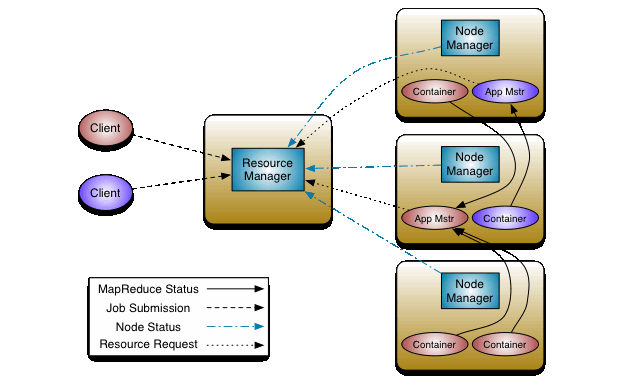
\includegraphics[width=.75\textwidth]{yarn_architecture.png}\\

\scriptsize\url{https://hadoop.apache.org/docs/current/hadoop-yarn/hadoop-yarn-site/yarn_architecture.gif}\normalsize
\caption{Executing MapReduce job on YARN cluster manager}
\label{fig:yarnhadoop}
\end{figure}

For a typical MapReduce application, the user specifies an input directory, possibly with multiple data files, to be processed. Recall that data files are distributed in blocks across the cluster node. A separate Map instance is executed for each input data block, on the node where the input data block is located. This means that any necessary program files are sent to a node as required. The shuffle phase sorts the output by key and moves data with the same key to the same node. While every instance of Reduce ''sees'' all values for the same key, a Reduce instance may process the values for multiple keys, depending on the number of unique key values and the number of nodes available in the cluster. 

\subsubsection*{Example}

While Hadoop MapReduce is natively programmed in Java, Hadoop Streaming allows Map and Reduce functions as executable programs, for example using Python. This example shows the basic operation of the Map and Reduce functions. The aim is to count the number of distinct words in a large text document. Both the Map and Reduce functions are implemented in Python. 

The Map function in the following Python code block reads lines from standard input. Hadoop Streaming is responsible for feeding those lines from the specified input to the Map function. After whitespace is stripped from the beginning and end of each line, the line is split into words. For each word, the Map outputs a key--value pair, separated by a tab character. The key is the word, the value is the number 1.

\begin{samepage}
\begin{pythoncode}
#!/usr/bin/env python
import sys

for line in sys.stdin:
    line = line.strip()
    words = line.split()
    for word in words:
        print ('{}\t{}'.format(word, 1))
\end{pythoncode}
\end{samepage}

Every instance of the Reduce function sees all values for a key, but may be processing the multiple keys. The following Reduce implementation reads key--value pairs from the standard input. It splits them on the tab character and maintains a dictionary of word counts. For each new key--value pair it increments its counter by the value it has just read. Finally, it outputs its results in the form of key--value pairs.

\begin{samepage}
\begin{pythoncode}
#!/usr/bin/env python
import sys

word_counts = dict()

for line in sys.stdin:
    word, count = line.split('\t', 1)
    count = int(count)

    if word not in word_counts:
       word_counts[word] = count
    else:
      word_counts[word] = word_counts[word] + count

for word, count in word_counts.items():
    print('{}\t{}'.format(word, count))
\end{pythoncode}
\end{samepage}

Before submitting this application as a job to a Hadoop cluster, it is useful to run it on the local machine and local filesystem. Download the program files and a data file and make the downloaded files executable:

\begin{samepage}
\begin{bashcode}
wget https://evermann.ca/busi4720/map.py
wget https://evermann.ca/busi4720/reduce.py
wget https://evermann.ca/busi4720/hamlet.txt
chmod +x *.py
\end{bashcode}
\end{samepage}

Then, run the Map function and view its output to understand how it works. The \texttt{''|''} symbol in the following bash code is a \emph{pipe} that pipes the output of one command into the next command. Here, the output of \texttt{cat}, which simply shows the contents of a file, are piped into the map function defined above, and its output is redirected with the \texttt{>} symbol to a file. The \texttt{less} command shows the contents of that file one line in an interactive way.

\begin{bashcode}
cat hamlet.txt | ./map.py > map.out
less map.out
\end{bashcode}

Next, run the Reduce function and view its output. The \texttt{sort} command sorts the content of text files. The \texttt{k2} option tells it that the sort key is the second column (word count) in the file, the \texttt{rn} option is to reverse the sort order (highest word count first).

\begin{bashcode}
cat map.out | ./reduce.py > reduce.out
sort -k2 -rn reduce.out | less
\end{bashcode}

Once the Map and Reduce functions work as expected on the local file system, they can be run on the Hadoop cluster. To do this, first put the input file(s) into their own directory on the HDFS:

\begin{bashcode}
hdfs dfs -mkdir hamlet
hdfs dfs -put hamlet.txt hamlet
hdfs dfs -ls hamlet
\end{bashcode}

Next, run the MapReduce application on the Hadoop cluster using Hadoop Streaming. The command arguments are self-explanatory, but note the use of the \texttt{file} arguments to tell Hadoop to move the program code to the nodes where the data are located. This illustrates the fundamental Hadoop principle that computation is moved to the data, not the other way around.

\begin{bashcode}
mapred streaming \
  -input hamlet -output hamlet.out \
  -mapper map.py -reducer reduce.py \
  -file map.py -file reduce.py
\end{bashcode}

The Hadoop cluster will now process the application, provide statistics and information about it as it is executed, and then report successful execution. The output directory, \texttt{hamlet.out} contains one result file from each instance of Reduce. 

Download the results to the local file system and sort and view them:

\begin{bashcode}
hdfs dfs -ls hamlet.out
hdfs dfs -get hamlet.out/part-*
cat part-* | sort -k2 -rn | less
\end{bashcode}

\newpage
\subsubsection*{Case Study}

\begin{wrapfigure}{l}{.2\textwidth}
\begin{center}

\includegraphics[width=.2\textwidth]{screen1.png}
\scriptsize \url{Source: IEEE}
\end{center}
\end{wrapfigure}
This case study illustrates the scalability of Hadoop in real business use case\footnote{Source: Evermann, J. (2016) Scalable Process Discovery using Map-Reduce. \emph{IEEE TSC}, 9 (3), 469-481. \url{https://doi.org/10.1109/TSC.2014.2367525}}. One aspect of business process mining is the discovery of process models from event logs. Event logs are generated by process-aware information systems and can grow to significant size. Event logs may be stored in a distributed way, either on those systems where they are generated, or in a dedicated business analytics Hadoop cluster. This suggests that a distributed implementation of process discovery algorithms using the MapReduce framework could provide significant scalability and performance advantages. 

The $\alpha$ miner and the Flexible Heuristics Minder (FHM) were implemented in MapReduce, the $\alpha$ miner requiring 2 Map--Reduce phases, while the FHM required 5 Map--Reduce phases. Expriments were conducted on a randomly generated process with 47 different types of activities. From this process, 5 million traces were simulated, yielding an event log of 80GB. To examine the effect of cluster size on performance, a single node cluster with 2 CPUs was chosen as a baseline and compared to a 10-node cluster with 2 CPUs on each node, and a 10-node cluster with 10 CPUs on each node. 

While the above word count example used simple data types for the keys and values, the data can be arbitrarily complex, as long as a function to compare keys is provided so that the shuffle phase can decide when two keys are the same and send values to the same Reduce instance. For example, the MapReduce implementation of the FHM used tuples of two elements for some keys and sets of multiple elements for some values:

\footnotesize
\begin{align*}
\text{map1:} &(Int, Text) \rightarrow set(CaseID, (Event, TimeStamp)) \\
\text{shuffle1:} &set(caseID, (Event, TimeStamp)) \rightarrow (CaseID, set(Event, TimeStamp)) \\
\text{reduce1:}  &(CaseID, set(Event, TimeStamp)) \rightarrow set((Event, Event), (Int, Bool, Int)) \\
\text{combine2:} &set((Event, Event), (Int, Bool, Int)) \rightarrow set((Event, Event, (Int, Bool, Int)) \\
\text{reduce2:}   &((Event, Event), set(Int, Bool, Int)) \rightarrow set(c, (Event, Event, Int, Float)) \\
\text{reduce3:}  & set(c, (Event, Event), set(Int, Float)) \rightarrow set(c, (Event, Event)) \\
\text{map4:}     & (Int, Text) \rightarrow set(CaseID, (Event, TimeStamp)) \\
\text{shuffle4:} & set(CaseID, (Event, TimeStamp)) \rightarrow (CaseID, set(Event, TimeStamp)) \\
\text{reduce4:}  & (CaseID, set(Event, TimeStamp)) \rightarrow set((Event, set(Event), Bool), Int) \\
\text{reduce5:}  & ((Event, set(Event), Bool), set(Int)) \rightarrow ((Event, set(Event), Bool), Int) 
\end{align*}
\normalsize

The experimental results, shown in Figure~\ref{fig:processdiscoveryresults} and Table~\ref{tab:processdiscoveryresults}, show the performance advantages delivered by parallel processing using multiple compute nodes with multiple CPUs each. Job completion time was reduced from days to minutes. 

\begin{figure}
\centering

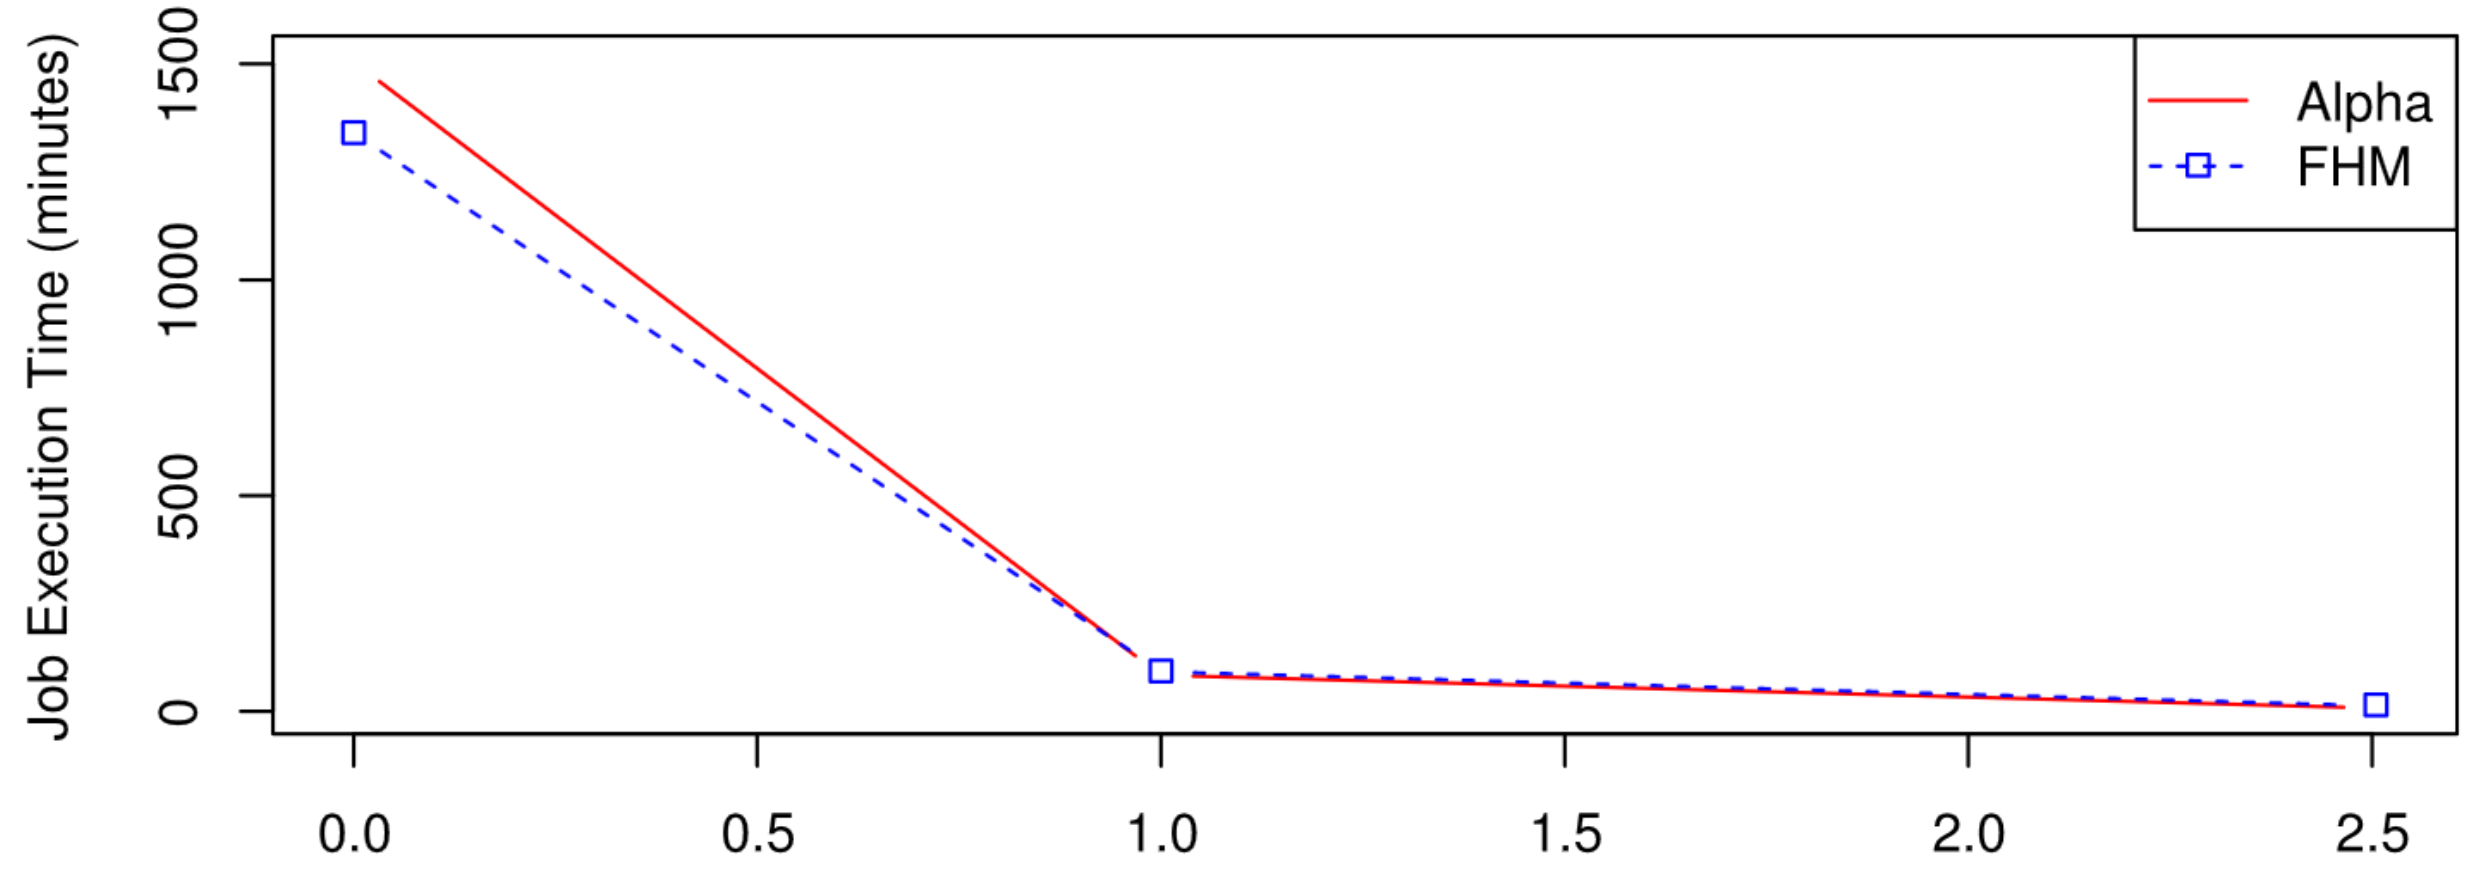
\includegraphics[width=.9\textwidth]{screen2.png} \\

\scriptsize
Source: Evermann, J. (2016) Scalable Process Discovery using Map-Reduce. \emph{IEEE TSC}, 9 (3), 469-481. \footnotesize \url{https://doi.org/10.1109/TSC.2014.2367525}
\caption[MapReduce performance for process discovery]{Total elapsed time for completion of MapReduce jobs for process discovery}
\label{fig:processdiscoveryresults}
\end{figure}

\begin{table}
\centering

\begin{tabular}{lr} \hline
\multicolumn{2}{c}{$\alpha$ Algorithm} \\
Single node & 25:00 hours \\
Medium cluster & 1:24 hours \\
Large cluster & 0:08 hours \\ \hline
\multicolumn{2}{c}{FHM} \\
Single node & 22:21 hours\\
Medium cluster & 2:01 hours \\
Large cluster & 0:17 hours \\ \hline
\end{tabular} \\

\vspace{\baselineskip}
\scriptsize
Source: Evermann, J. (2016) Scalable Process Discovery using Map-Reduce. \emph{IEEE TSC}, 9 (3), 469-481. \footnotesize \url{https://doi.org/10.1109/TSC.2014.2367525}
\caption[MapReduce performance for process discovery]{Total elapsed time for completion of MapReduce jobs for process discovery}
\label{tab:processdiscoveryresults}
\end{table}

\FloatBarrier
\subsubsection*{Apache Pig}

\begin{wrapfigure}{l}{.25\textwidth}
\begin{center}

\includegraphics[width=.25\textwidth]{pig_logo.png} \\
\tiny\url{https://en.wikipedia.org/wiki/File:Apache_Pig_Logo.svg}
\end{center}
\end{wrapfigure}
Apache Pig\footnote{\url{https://pig.apache.org/docs/latest/basic.html}} is a high-level platform for creating programs that run on Apache Hadoop. It is designed to simplify the complexities of writing low-level MapReduce programs, providing a simpler scripting language called Pig Latin, which abstracts the details of programming from the underlying MapReduce framework. Apache Pig was originally developed at Yahoo to allow analysts using Hadoop to focus more on analyzing large data sets and spend less time having to write Map and Reduce functions. Although it operates at a higher level of abstraction than MapReduce, under the hood, Pig converts these scripts into MapReduce jobs.

Pig Latin is designed to handle all kinds of data, particularly semi-structured data or datasets that do not conform to a fixed schema. Pig Latin supports operations like join, sort, filter, and combine but is tailored to handle complex nested data structures typical in big data applications. Users can extend the language with their own functions written in Java, JavaScript, Python, etc., to handle custom processing. Typically, Pig Latin programs are about 5-20 times shorter than equivalent Java MapReduce programs. However, Pig Latin remains a procedural language, focusing on how to retrieve or process data, rather than a declarative langauage like SQL that focuses on what data to retrieve. Table~\ref{tab:pigoperators} shows the core relational operations available in Pig Latin.

To give an impression of Pig Latin, consider the following script\footnote{\small Source: \url{https://en.wikipedia.org/wiki/Apache_Pig}} that performs the same word count as the MapReduce example above.

\begin{sqlcode}
input_lines = LOAD 'hamlet.txt' AS (line:chararray);
-- Extract words from each line and put them into 
-- a pig bag datatype, then flatten the bag to get
-- one word on each row
words = FOREACH input_lines \
   GENERATE FLATTEN(TOKENIZE(line)) AS word;
-- create a group for each word
word_groups = GROUP words BY word;
-- count the entries in each group
word_count = FOREACH word_groups  \
   GENERATE COUNT(words) AS count, group AS word;
-- order the records by count
ordered_word_count = ORDER word_count BY count DESC;
STORE ordered_word_count INTO 'hamlet.out';
\end{sqlcode}

\begin{table}
\centering

\renewcommand{\arraystretch}{1.5}
\begin{tabular}{ccccc} 
LOAD & STORE & DUMP & FILTER & DISTINCT \\
FOREACH $\ldots$ GENERATE & UNION & SAMPLE & JOIN & GROUP \\
CROSS & ORDER & LIMIT & SPLIT \\
\end{tabular}
\caption{Core Pig Latin operations}
\label{tab:pigoperators}
\end{table}


\subsubsection*{Apache Hive}

\begin{wrapfigure}{l}{.25\textwidth}
\begin{center}

\includegraphics[width=.25\textwidth]{hive_logo.png} \\
\tiny\url{https://commons.wikimedia.org/wiki/File:Apache_Hive_logo.svg}
\end{center}
\end{wrapfigure}
Apache Hive is a data warehousing software and SQL-like query language for data stored on Hadoop's HDFS. Hive is designed to make Hadoop accessible to business analysts familiar with SQL, the standard language for relational databases. However, Hive is not a full database. The main focus is to provide data summarization, query, and analysis. While it has similar properties to a database, such as indexing, transactions, and queries, it does not offer real-time queries and row-level updates.

HiveQL\footnote{\url{https://cwiki.apache.org/confluence/display/Hive/LanguageManual}} is the SQL-like language that Hive uses. HiveQL includes extensions that allow traditional MapReduce programmers to plug in their custom Map and Reduce functions when it is inconvenient or inefficient to express this logic in HiveQL. Hive reduces the complexity of writing MapReduce jobs by automatically translating HiveSQL queries into MapReduce jobs, allowing users to focus on query statements rather than the complexities of the underlying execution engines.

Consider the following example HiveQL query\footnote{\small Source: \url{https://en.wikipedia.org/wiki/Apache_Hive}}. It imeplements the same word count as the above Pig Latin script and the earlier MapReduce example. Note the similarities to SQL and the declarative nature. The HiveQL query does not specify what actions to perform, but simply specifies what result to retrieve or select from the data set. 

\begin{sqlcode}
DROP TABLE IF EXISTS docs;
CREATE TABLE docs (line STRING);
LOAD DATA INPATH 'hamlet.txt' 
  OVERWRITE INTO TABLE docs;
  
CREATE TABLE word_counts AS
SELECT word, count(1) AS count FROM
  (SELECT explode(split(line, '\s')) 
    AS word FROM docs) temp
GROUP BY word
ORDER BY word;
\end{sqlcode}

\section{Apache Spark}

\begin{wrapfigure}{l}{.25\textwidth}
\begin{center}

\includegraphics[width=.25\textwidth]{spark_logo.png}
\tiny \url{https://commons.wikimedia.org/wiki/File:Apache_Spark_logo.svg} \normalsize
\end{center}
\end{wrapfigure}
Apache Spark is an open-source, unified analytics system for large-scale data processing. Originally designed at developed at the University of California at Berkeley in 2009, it was donated as an open-source project to the Apache Foundation in 2013. It provides high-level programming interfaces for Java, Scala, Python, and R. It is known for its speed and ease of use in complex analytics across big data. Because of its advantages over Hadoop and MapReduce, it was quickly adopted.

Spark's core feature is its in-memory cluster computing that increases the processing speed of an application significantly over MapReduce, which is disk limited. Spark stores data in RAM across the cluster, which allows it to access this data quickly and speed up the computation times, especially for iterative algorithms common in machine learning and data mining. In contrast to MapReduce, Spark also supports cyclic data flow.

Spark can run on top of existing Hadoop clusters to leverage Hadoop's storage systems, like HDFS or HBase. This allows for easy integration and migration of data-processing tasks between Hadoop components and Spark. Like Hadoop, Spark is designed to scale up from a single server to thousands of machines, each offering local computation and storage. However, Spark can also use cloud-based file storage such as Amazon Web Services S3 or Microsoft Azure storage solutions, and cluster management software other than YARN, such as Mesos or Kubernetes.

Spark provides a unified processing engine that can handle different types of workloads within the same application that have traditionally required separate distributed systems, including batch processing, SQL queries, real-time stream processing, machine learning, and graph processing. This unification reduces management overhead and streamlines data processing pipelines.

Spark uses a data storage model based on RDDs (Resilient Distributed Datasets), which are automatically rebuilt on cluster node failure. This design ensures that Spark applications can handle node failures on large clusters with minimal impact on data processing tasks.

Spark's easy-to-use programming interface simplify the development of complex, multi-stage data pipelines and sophisticated analytics and machine learning compared to MapReduce. Spark also includes Spark SQL, making it easy to transition from traditional SQL databases to big data processing.

Figure~\ref{fig:sparkcomponents} shows the components of Spark. Despite its name, Spark SQL also provides more traditional data frame operations, similar to those one might see in the Python Pandas or R Tidyverse packages. 

\begin{figure}
\centering

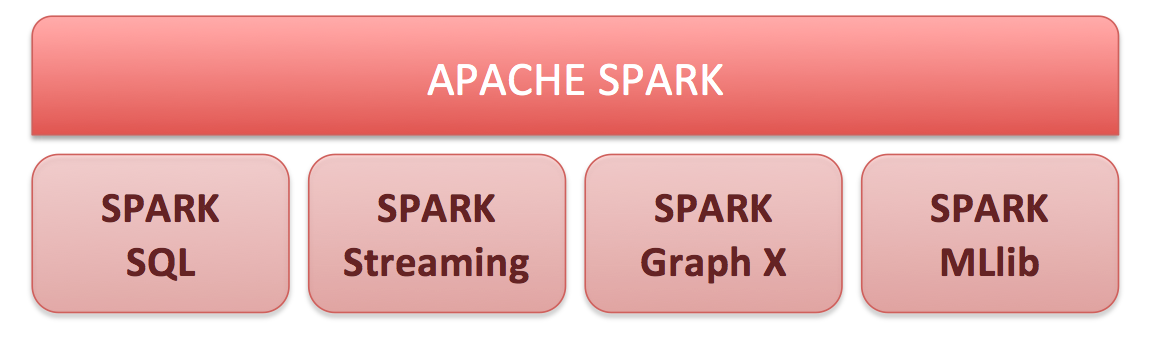
\includegraphics[width=.75\textwidth]{spark_components.png}
\scriptsize \url{https://commons.wikimedia.org/wiki/File:Sch\%C3\%A9ma_d\%C3\%A9tail_outils_spark.png} \normalsize
\caption{Apache Spark components}
\label{fig:sparkcomponents}
\end{figure}

\begin{tcolorbox}[colback=code]
The Apache Spark web site provides a wealth of information, both at the introductory, conceptual level and the advanced, detailed level. The following sections are useful for learning more about Apache Spark:

\begin{itemize}
\item \href{https://spark.apache.org/docs/latest/quick-start.html}{Quick Start}
\item \href{https://spark.apache.org/docs/latest/sql-programming-guide.html}{SQL, DataFrames and Datasets}
\item \href{https://spark.apache.org/docs/latest/structured-streaming-programming-guide.html}{Structured Streaming}
\item \href{https://spark.apache.org/docs/latest/ml-guide.html}{Machine Learning}
\end{itemize}
\end{tcolorbox}

\subsubsection*{Cluster Management}

Apache Spark provides its own cluster management, shown in Figure~\ref{fig:sparkcluster}. An analytics application (''driver program'') uses a Spark context to communicate with the Spark cluster manager. The cluster manager in turn coordinates and controls the worker nodes. Worker nodes run on each computer in the cluster to manage the local resources and execute tasks. When a client application requests execution of a Spark job via the Spark context, the cluster manager assigns worker nodes and their executors to the different tasks in the job. The executors execute the assigned tasks and communicate with the Spark context of the client application for status updates and results.

\begin{figure}
\centering

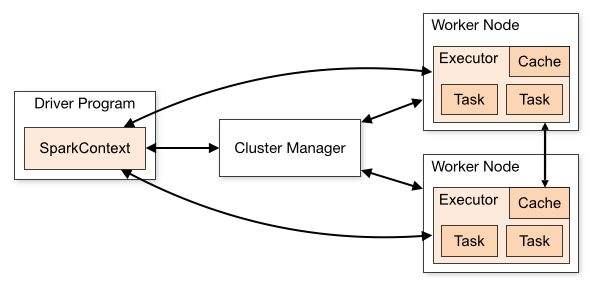
\includegraphics[width=.75\textwidth]{cluster-overview.png}
\scriptsize \url{https://spark.apache.org/docs/latest/img/cluster-overview.png}
\caption{Apache Spark cluster architecture}
\label{fig:sparkcluster}
\end{figure}

\subsection{Spark SQL}

Despite the name ''Spark SQL'', this component of Spark also offers non-SQL based data management. This section first describes three different kinds of data storage in Spark, introduces execution of transformations and actions on them, then provides some basic examples, and finally illustrates the use of SQL in Spark.

\subsubsection*{Data Storage Architecture}

The fundamental data structure of Apache Spark is the Resilient Distributed Dataset (RDD). RDDs are designed to provide a fault-tolerant, immutable collection of objects that can be processed in parallel. An RDD can contain any type of Python, Java, or Scala data objects. RDDs are immutable, that is, once created they cannot be changed. Data in RDDs is split into logical partitions, which can be processed on different nodes of the cluster. RDDs achieve resilience, that is, fault tolerance, through a lineage graph of the input dataset --- each RDD ''remembers'' how to reconstruct its segments from other datasets by logging the transformations used to build it from other RDDs.

When Apache Spark is run on a Hadoop cluster, RDDs are created from data stored in HDFS. Spark builds the RDD partitions directly from the blocks of the corresponding file stored on the HDFS. This direct alignment allows Spark to leverage HDFS's location model, which places computations near the data. Since RDD partitions correspond to HDFS blocks, operations on RDDs can be scaled across many nodes, allowing Spark to leverage the distributed nature of the HDFS architecture to process large datasets in parallel. The correspondence of Spark RDD partitions and HDFS blocks also means there are two layers of fault tolerance. First, the HDFS replication ensures that data can be recovered in case of node failure from another replica. Second, the Spark RDD lineage information means the RDD can be re-computed from its inputs given its history. RDDs offer a low-level programming interface that is focused on MapReduce. It is procedural and offers no optimization of query operations. 

Building on RDDs, Spark provides DataFrames and Datasets that provide a high-level, more abstract programming interface similar to Python Pandas data frames or R dataframes. A DataFrame in Spark is a distributed collection of data organized into named columns. Spark DataFrames use a query optimizer to optimize the execution of DataFrame queries for better performance. DataFrames support various data formats and data sources, including JSON, CSV, and relational databases. DataFrames are also integrated with Spark SQL for running SQL queries.

Datasets in Spark are an extension of DataFrames that provide a type-safe, object-oriented programming interface. Datasets are only available in the Scala and Java programming languages; the Python and R programming languages do not have the type information required to use them.

\subsubsection*{Spark Execution Principles}

Apache Spark's core programming model for DataFrames and Datasets revolves around transformations and actions. These operations adhere to the principle of lazy execution, which is fundamental to Spark's high performance and efficiency in processing large datasets.

\begin{table}
\renewcommand{\arraystretch}{1.25}

\begin{tabularx}{\textwidth}{l|X} \hline
\texttt{select()} & Projects a set of expressions and returns a new DataFrame. \\
\texttt{filter()} or \texttt{where()} & Filters rows using the given condition and returns a new DataFrame with only the satisfying rows. \\
\texttt{groupBy()} & Groups the DataFrame using the specified columns, so that further aggregation can be performed. \\
\texttt{join()} & Joins with another DataFrame, using the given join expression. \\
\texttt{orderBy()} or \texttt{sort()} & Returns a new DataFrame sorted by the specified column(s).\\
\texttt{drop()} & Removes a column or columns from a DataFrame.\\
\texttt{withColumn()} & Returns a new DataFrame by adding a column or replacing an existing column that has the same name.\\
\texttt{withColumnRenamed()} & Renames a column in the DataFrame. \\
\texttt{distinct()} & Returns a new DataFrame containin the distinct rows of the source DataFrame.\\
\texttt{union()} & Combines two DataFrames that have the same schema, appending the rows of one DataFrame to another.\\
\texttt{cov()} & Covariance of columns in a DataFrame.\\ \hline
\end{tabularx}
\caption{Common Spark DataFrame transformations}
\label{tab:sparktransformations}
\end{table}


\emph{Transformations} are operations that create a new DataFrame from an existing one. They are considered ''\emph{lazy}'', meaning that they do not compute their results right away. Instead, Spark maintains a plan (the ''lineage'') of all transformations applied to the DataFrame. Common transformations on DataFrames are listed in Table~\ref{tab:sparktransformations}. Transformations are only executed when an \emph{action} is applied to the DataFrame. This approach allows Spark to optimize data processing, for example by internally rearranging or combining operations.

\emph{Actions} are operations that trigger computation and return results from a DataFrame to the client application or write results to storage. Examples of actions are shown in Table~\ref{tab:sparkactions}. When an action is called on a DataFrame, Spark evaluates the DataFrame transformations that have been built up in the lineage. It then optimizes the execution plan for these transformations and executes the different tasks across the cluster to compute the final results.

\begin{table}
\renewcommand{\arraystretch}{1.25}

\begin{tabularx}{\textwidth}{l|X} \hline
\texttt{show()} & Displays the contents of the DataFrame in tabular form.\\
\texttt{count()} & Returns the number of rows in the DataFrame.\\
\texttt{collect()} & Retrieves the entire DataFrame and returns it as a collection of rows on the driver program.\\
\texttt{save()} & Saves the DataFrame to an external storage system, such as HDFS or a local filesystem.\\
\texttt{take(n)} & Returns an array with the first n rows in the DataFrame.\\
\texttt{head()} & Retrieves the first $n$ rows of a DataFrame.\\
\texttt{tail()} & Retrieves the last $n$ rows of a DataFrame.\\
\texttt{toPandas()} & Converts a Spark DataFrame to a Pandas DataFrame, bringing the entire data set into memory.\\
\texttt{write.csv()} & Writes the contents of a DataFrame to a CSV file.\\ \hline
\end{tabularx}
\caption{Common Spark DataFrame actions}
\label{tab:sparkactions}
\end{table}

\subsubsection*{Basic Examples}

The examples in this section are intended to illustrate the basic usage of Spark on a Hadoop cluster. They assume that Spark is running on a Hadoop cluster with HDFS storage. They use Python and the PySpark interactive console.

First, start the local Hadoop cluster (if not already running) and the PySpark console. PySpark is Python with a built-in Spark context object to connect to the cluster manager, as shown in the output below. The Hadoop YARN cluster manager manages the PySpark application, and has a web interface at \url{localhost:8088}. From there, information about the PySparkShell application can be viewed.

\begin{samepage}
\begin{bashcode}
sudo systemctl start hadoop.service
pyspark --master yarn
\end{bashcode}
\end{samepage}

The result is the PySparkShell, which is a Python shell with a Spark context object that provides the connection to the cluster manager:

\begin{samepage}
\begin{textcode}
Python 3.10.12 (main, Nov 20 2023, 15:14:05) [GCC 11.4.0] on linux
Type "help", "copyright", "credits" or "license" for more information.
Welcome to
      ____              __
     / __/__  ___ _____/ /__
    _\ \/ _ \/ _ `/ __/  '_/
   /__ / .__/\_,_/_/ /_/\_\   version 3.5.1
      /_/

Using Python version 3.10.12 (main, Nov 20 2023 15:14:05)
Spark context Web UI available at http://10.0.2.15:4040
Spark context available as 'sc' (master = yarn, app id = application_
SparkSession available as 'spark'.
\end{textcode}
\end{samepage}

The following Python code block reads a file from HDFS and gathers some statistics. Note that the \texttt{textFile} is treated as a DataFrame with typical data frame operations such as \texttt{count()} and \texttt{filter()}. PySpark will provide some information about the job progress on the cluster as these operations are executed.

\begin{samepage}
\begin{pythoncode}
textFile = spark.read.text(\
    'hdfs://localhost:9000/user/busi4720/hamlet.txt')
# Number of lines
textFile.count() 
# First row
textFile.first()
# How many lines contain the word Hamlet?
textFile.filter(textFile.value.contains("Hamlet")).count() 
\end{pythoncode}
\end{samepage}

The Python code block below shows another example of Spark DataFrame operations. It finds the longest line by number of words. It imports a number of useful functions from the Spark SQL package. The \texttt{sf.split()} function splits a character string on a regular expression into a list of words, \texttt{sf.size()} returns the length of that list, \texttt{sf.col()} returns a specified columns, and the \texttt{sf.max()} function returns the maximum of its arguments. The \texttt{agg()} function specifies an aggregation and the final \texttt{collect()} is an action that triggers execution of the transformation operations.

\begin{samepage}
\begin{pythoncode}
# Import useful functions from Spark SQL:
from pyspark.sql import functions as sf
# Split each line and count words as 'numWord', 
# then aggregate the 'numWords' columns using 'max':
textFile.select(sf.size(sf.split(textFile.value, "\s+")) \
    .alias("numWords")) \
    .agg(sf.max(sf.col("numWords"))) \
    .collect()
\end{pythoncode}
\end{samepage}

The following Python code block implements the word count. It uses two functions from the Spark SQL library, \texttt{sf.split()} and \texttt{sf.explode()}. The first splits a line of text (a character string) on a regular expression, here, one or more whitespace characters. The \texttt{sf.explode()} function converts the list resulting from \texttt{sf.split()} into a DataFrame column. This column is then called ''word''. The \texttt{groupBy()} and \texttt{count()} operations then aggregate the information. The final \texttt{collect()} is an action that triggers actual execution of the transformation operations.

\begin{samepage}
\begin{pythoncode}
# Import useful functions from Spark SQL:
from pyspark.sql import functions as sf

wordCounts = textFile \
    .select(sf.explode(sf.split(textFile.value, "\s+")) \
    .alias("word")) \
    .groupBy("word") \
    .count() \
    .orderBy("count")
wordCounts.collect()
\end{pythoncode}
\end{samepage}

\subsubsection*{Spark Schemas}

In Apache Spark, a schema is a structured definition of the columns and their data types in a DataFrame. Schemas serve several important purposes when creating or reading a DataFrame. First, schemas are used to validate the data, ensuring that the data matches the expected format and types. Second, knowing the schema avoids the overhead of inferring data types and enables better optimization techniques. 

Spark supports a variety of data types similar to traditional database types, which are used to define the columns in a DataFrame. Common data types in Spark are 'Integer', 'Long', 'Double', 'Float', 'String', 'Boolean', 'Timestamp', 'Date', 'Smallint', 'Tinyint', 'Bigint', and the complex types 'Struct', 'Array' and 'Map'.

A schema in Spark is defined using the Spark schema DDL (data definition language) which looks superficially like an SQL table definition, as shown in the following PySpark example that defines a schema for reading an event log file for process analytics:

\begin{samepage}
\begin{pythoncode}
# Define a schema using Spark schema DDL
logSchema = \
    'caseID STRING, \
     activity STRING, \
     ts TIMESTAMP'
\end{pythoncode}
\end{samepage}

The schema can then be used the reading data into a DataFrame, as shown in the Python code block below. A CSV file is read from HDFS using specific options for delimiter and header row and the schema defined above:

\begin{samepage}
\begin{pythoncode}
fname='hdfs://localhost:9000/user/busi4720/eventlog.short.log'

data = spark.read \
    .format('csv') \
    .option('delimiter', '\t') \
    .option('header', 'false') \
    .schema(logSchema) \
    .load(fname)
\end{pythoncode}
\end{samepage}

The following PySpark commands provide basic information for the DataFrame:

\begin{samepage}
\begin{pythoncode}
data.printSchema()
data.count()
data.show(5)
data.summary().show()
\end{pythoncode}
\end{samepage}

\subsubsection*{Spark SQL}

The word count example above used DataFrame operations similar to those in R or Pandas on Spark DataFrames. Another way to work with DataFrames is to treat them as a table and use SQL queries.

DataFrames can be turned into temporary tables, called ''views''. These are not physically recorded and are lost when the PySpark application ends (or the view is explicitly destroyed).

\begin{pythoncode}
data.createOrReplaceTempView('log')
\end{pythoncode}

Alternatively, a DataFrame can written to a permanent table. This table persists in Hadoop storage beyond the PySpark application:

\begin{pythoncode}
data.write.saveAsTable('log_table')
\end{pythoncode}

In either case, the \texttt{spark.sql()} function allows the use of SQL commands on the temporary or permanent table:

\begin{samepage}
\begin{pythoncode}
result_df = spark.sql('select * from log limit 5')
result_df.show()
\end{pythoncode}
\end{samepage}

For a more elaborate example, consider the construction of a Directly-Follows-Graph (DFG), as used in business process analytics. This is relatively easy to do with the follwing SQL query. It computes the number of times an activity directly follows another activity, as well as the mean time between two activities following each other. 

\begin{samepage}
\begin{pythoncode}
sql_query = \
'SELECT COUNT(*), l1.activity AS activity1, \
 l2.activity AS activity2, AVG(l2.ts - l1.ts) AS dtime \
  FROM log AS l1 JOIN log AS l2 ON l1.caseid=l2.caseid \
   WHERE l2.ts = (SELECT MIN(ts) FROM log l3 \
    WHERE l3.caseid=l1.caseid AND l3.ts > l1.ts) \
     GROUP BY GROUPING SETS((l1.activity, l2.activity))'
\end{pythoncode}
\end{samepage}

Query execution may require some time due to the multiple self-joins on the log table. 

\begin{samepage}
\begin{pythoncode}
# Run the query, show the results
dfg = spark.sql(sql_query)
dfg.count()
dfg.show()
\end{pythoncode}
\end{samepage}

To illustrate the concept of a query plan and query plan optimization, it may be useful to examine the optimized query plan that Spark uses for the actual calculations. The output provides information about the logical query plans, both the initial and the optimized one, as well as the physical query plan, the set of tasks that Spark runs on the cluster nodes to calculate the result.

\begin{samepage}
\begin{pythoncode}
# Explain the query plan:
dfg.explain(mode='formatted')
dfg.explain(True)
\end{pythoncode}
\end{samepage}

So far, the Spark examples have been run interactively from the PySpark console. However, longer running analytics jobs are typically submitted to the Spark cluster for execution as self-contained applications so the analyst does not have to wait for results to be returned. To do this, one can use the \texttt{spark-submit} command and specify the PySpark file and its arguments. The following example downloads a Python application file (which contains the above code to compute the DFG) and then submits it to the cluster manager for execution, providing the HDFS file name as its argument. Result will be written to HDFS. While the job is running, use Hadoop Job Tracker at \url{https://localhost:8088} to track the status of nodes and the progress of jobs.

\begin{samepage}
\begin{bashcode}
# Download file
wget https://evermann.ca/busi4720/spark_dfg.py
# Submit to Spark/Hadoop cluster
spark-submit --master yarn spark_dfg.py \
 hdfs://localhost:9000/user/busi4720/eventlog.short.log
\end{bashcode}
\end{samepage}

\subsection{Spark Machine Learning}

Apache Spark provides support for machine learning through its MLlib and Spark ML libraries. Both libraries offer common learning algorithms like classification (logistic regression, decision trees, support vector machines, random forests, etc.), regression (generalized linear regression, regression trees, etc.), and clustering (for example, k-means). Utilities for feature extraction, transformation, dimensionality reduction (for example, PCA), and feature selection are provided to prepare data for machine learning models. MLlib and Spark ML support the concept of pipelines, which simplify the process of transforming data and tuning parameters. Models and algorithms can be saved to and loaded from storage, facilitating the reuse and application of models across different applications and frameworks. Spark ML provides a higher-level programming interface built on DataFrames for constructing ML pipelines, whereas MLlib is the original machine learning library for Spark and is based on RDDs. Spark ML is the primary focus of development; while still supported, MLlib receives less attention in terms of new features or performance improvements.

In Apache Spark ML, the concepts of pipelines, transformers, and estimators are central to defining data transformations and machine learning workflows in a reusable, manageable way. A \emph{pipeline} in Spark ML represents a workflow that consists of a sequence of stages, each of which is either a \emph{transformer} or an \emph{estimator}. These stages are executed in order and transform the input DataFrame as it passes through each stage. Once a pipeline is defined, it acts like an estimator. Running the pipeline's \texttt{fit()} method on a DataFrame produces a fitted model (''PipelineModel''), which is a Transformer.

\emph{Transformers} take a DataFrame as input and return a new DataFrame with more features or a different arrangement of features as output. Common examples of transformers are the 'Tokenizer' that splits text into words, the 'StringIndexer' that converts a column of labels to a column of integer indices, or the 'VectorAssembler' that combines multiple columns into a single vector.

An \emph{Estimators} represents a learning algorithms that fits or trains on data. Estimators provide a \texttt{fit()} method, which accepts a DataFrame and produces a model, which in turn is a Transformer. Common examples of Estimators include 'LogisticRegression', 'DecisionTreeClassifier' or ''KMeans'.

Figure~\ref{fig:sparkpipelines} illustrates the use of Spark ML pipelines. The upper panel shows a pipeline consisting of two transformers (blue), followed by an estimator (red). Once the \texttt{fit()} method of the pipeline is called, the estimator (and the entire pipeline) become a transformer (blue). The lower panel shows that this fitted/trained transformer pipeline can then be used to transform input into predictions. 

\begin{figure}
\centering

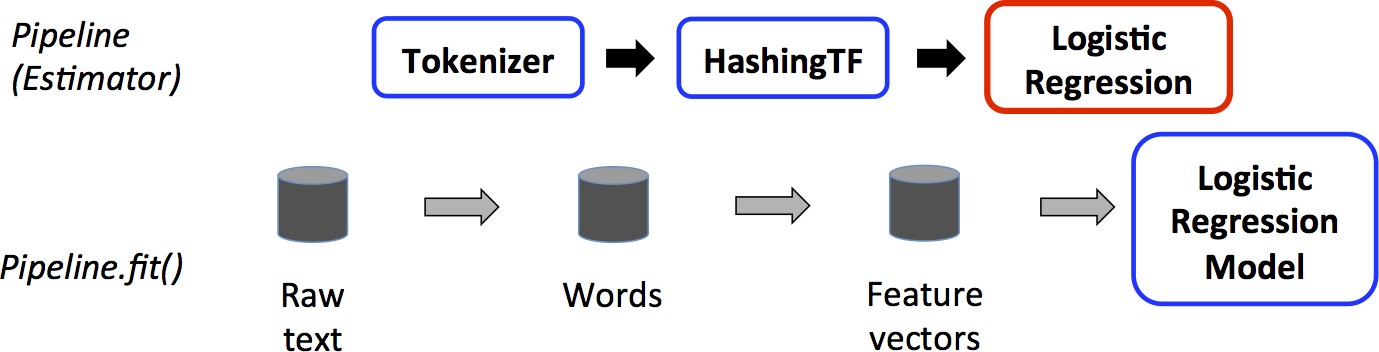
\includegraphics[width=.75\textwidth]{ml-Pipeline1.png} 

\vspace{.5\baselineskip}
\rule{.75\textwidth}{.5pt}
\vspace{.5\baselineskip}

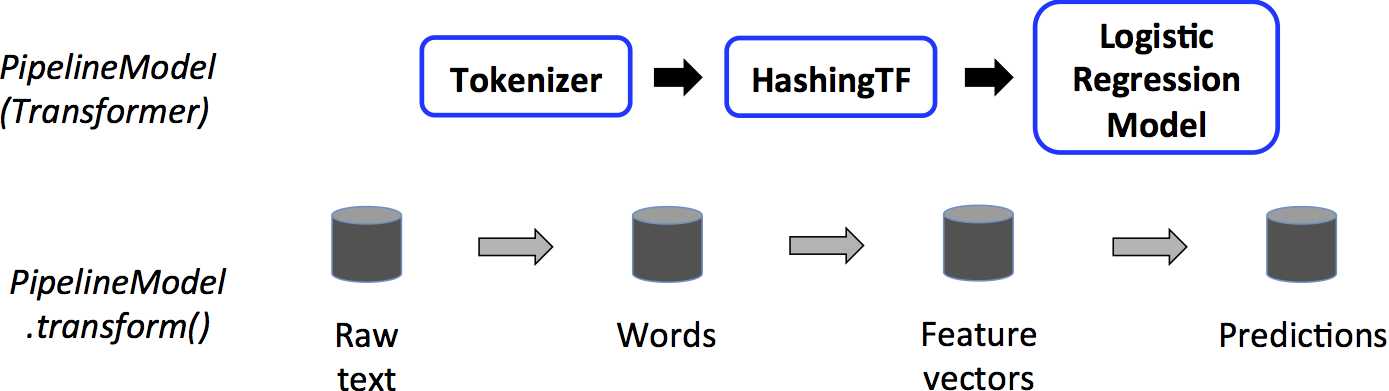
\includegraphics[width=.75\textwidth]{ml-Pipeline2.png} 

\scriptsize Source: \url{https://spark.apache.org/docs/latest/ml-pipeline.html} \normalsize
\caption{Pipelines in Spark ML}
\label{fig:sparkpipelines}
\end{figure}

The following example illustrates the use of Spark ML for binary classification. The example requires some feature transformation to illustrate the use of the pipelines. The full example is available to run as self-contained application\footnote{\url{https://evermann.ca/busi4720/spark_ml.py}} using \texttt{spark-submit} on a Spark cluster. Remember that the Hadoop job tracker\footnote{\url{https://localhost:8080}} is available to track the status of the submitted Spark job. The data set for this example is a public dataset originally from the UCI mchine learning laboratory\footnote{Source: \url{https://archive.ics.uci.edu/dataset/848/secondary+mushroom+dataset}, CC-BY 4.0 license}.

\begin{samepage}
\begin{bashcode}
# Download file
wget https://evermann.ca/busi4720/spark_ml.py

# Get the dataset and put on HDFS
wget https://evermann.ca/busi4720/mushrooms.csv
hdfs dfs -put mushrooms.csv

# Submit to Spark/Hadoop cluster
spark-submit --master yarn spark_ml.py \
    hdfs://localhost:9000/user/busi4720/mushrooms.csv
\end{bashcode}
\end{samepage}

The remainder of this section illustrates the code in detail. First, the schema is defined for reading the CSV data set into a Spark DataFrame and to validate the data types:

\begin{samepage}
\begin{pythoncode}
the_schema = 'class STRING, `cap-diameter` DOUBLE, \
    `cap-shape` STRING, `cap-surface` STRING, \
    `cap-color` STRING, `does-bruise-or-bleed` STRING, \
    `gill-attachment` STRING, `gill-spacing` STRING, \
    `gill-color` STRING, `stem-height` DOUBLE, \
    `stem-width` DOUBLE, `stem-root` STRING, \
    `stem-surface` STRING, `stem-color` STRING, \
    `veil-type` STRING, `veil-color` STRING, \
    `has-ring` STRING, `ring-type` STRING, \
    `spore-print-color` STRING, habitat STRING, \
    season STRING'
\end{pythoncode}
\end{samepage}

The \texttt{spark.read()} function uses the schema and specific parameters for delimiter and header rows to read the CSV file into a Spark DataFrame. The ''veil-type'' column is then dropped and missing values are replaced by the character string 'NULL'.

\begin{samepage}
\begin{pythoncode}
fname='hdfs://localhost:9000/user/busi4720/mushrooms.csv'

data = spark.read \
    .format('csv') \
    .option('delimiter', ',') \
    .option('header', 'true') \
    .schema(the_schema) \
    .load(fname)
data = data.drop('veil-type')
data = data.fillna('NULL')
\end{pythoncode}
\end{samepage}

\begin{samepage}
Next, import the required packages:
\begin{pythoncode}
# Import all required pieces:
from pyspark.ml import Pipeline
from pyspark.ml.classification import LogisticRegression
from pyspark.ml.feature import StandardScaler, \
    StringIndexer, OneHotEncoder, VectorAssembler
from pyspark.ml.evaluation import BinaryClassificationEvaluator
from pyspark.ml import PipelineModel
\end{pythoncode}
\end{samepage}

\begin{samepage}
The numerical feature columns are concatenated (''assembled'') into a single vector column using the \texttt{VectorAssembler} transformer:
\begin{pythoncode}
numFeatures = VectorAssembler(
    inputCols = ['cap-diameter', 'stem-width', 'stem-height'],
    outputCol = 'numFeatures')
\end{pythoncode}
\end{samepage}

\begin{samepage}
The \texttt{StandardScaler} transformer scales and standardizes the numerical features:
\begin{pythoncode}
scaler = StandardScaler(inputCol='numFeatures',
                        outputCol='numFeaturesS')
\end{pythoncode}
\end{samepage}

The categorical variables are one-hot encoded using dummy variables. First, identify the columns with 'string' data type, and construct column names for the indexed and one-hot encoded corresponding columns:

\begin{samepage}
\begin{pythoncode}
categoricalCols = \
    [name for (name, dtype) in data.dtypes if dtype=='string']
indexOutputCols = [x + 'index' for x in categoricalCols]
oheOutputCols = [x + 'ohe' for x in categoricalCols]
\end{pythoncode}
\end{samepage}

A \texttt{StringIndexer} is a transformer that transforms a column or set of columns of character strings into a column or set of columns of integer indices.

\begin{samepage}
\begin{pythoncode}
stringIndexer = StringIndexer(
    inputCols = categoricalCols,
    outputCols = indexOutputCols,
    handleInvalid='skip')
\end{pythoncode}
\end{samepage}

The \texttt{OneHotEncoder} takes one or more numerical category index columns and returns the corresponding one-hot encoded columns:

\begin{samepage}
\begin{pythoncode}
oheEncoder = OneHotEncoder(
    inputCols = indexOutputCols,
    outputCols = oheOutputCols)
\end{pythoncode}
\end{samepage}

Finally, the numerical and categorical feature columns are combined into a column with the entire feature vector using another \texttt{VectorAssembler} transformer:

\begin{samepage}
\begin{pythoncode}
# Assemble all features into a feature vector
vecAssembler = VectorAssembler(
    inputCols = oheOutputCols+['numFeaturesS'],
    outputCol = 'feature_vec')
\end{pythoncode}
\end{samepage}

The targets are also encoded as numerical indices, using the \texttt{StringIndexer} transformer:

\begin{samepage}
\begin{pythoncode}
# Encode the target classes as numbers
stringIndexTarget = StringIndexer(
    inputCols = ['class'],
    outputCols = ['classIndex'],
    handleInvalid='skip')
\end{pythoncode}    
\end{samepage}

As the last required element, the \texttt{LogisticRegression} estimator is defined, accepting the feature vector column and the target column:

\begin{samepage}
\begin{pythoncode}
# Create the classification estimator
logReg = LogisticRegression(
    featuresCol = 'feature_vec', labelCol = 'classIndex')
\end{pythoncode}
\end{samepage}
All components can be assembled into a pipeline:

\begin{samepage}
\begin{pythoncode}
# Put all components into the pipeline
pipeline = Pipeline(stages=[
    numFeatures,
    scaler,
    stringIndexer,
    oheEncoder,
    vecAssembler,
    stringIndexTarget,
    logReg])
\end{pythoncode}
\end{samepage}

To train the model, the data set is split into training and test data, using the \texttt{randomSplit} transformation on the Spark DataFrame:

\begin{samepage}
\begin{pythoncode}
# Create train/test data split
train_data, test_data = data.randomSplit([.66, .33], seed=1)
\end{pythoncode}
\end{samepage}

Calling the pipeline's \texttt{fit} method will turn the final estimator, and the entire pipeline into a fitted model, that is, a transformer:

\begin{samepage}
\begin{pythoncode}
# Fit the model to the training data
pipelineModel = pipeline.fit(train_data)
\end{pythoncode}
\end{samepage}

Performance metrics for the training data can be retrieved from the last stage of the pipeline, that is, from the \texttt{LogisticRegression} estimator (now a transformer):

\begin{samepage}
\begin{pythoncode}
# Summary of the training data performance
summary = pipelineModel.stages[-1].summary
summary.accuracy
summary.areaUnderROC
summary.fMeasureByThreshold.show()
summary.precisionByLabel
summary.recallByLabel
summary.roc.show()
\end{pythoncode}
\end{samepage}

Fitted estimators, including whole pipelines, become transformers. The \texttt{transform()} method of a transformer can be used to transform inputs into output predictions: 

\begin{samepage}
\begin{pythoncode}
trainPred = pipelineModel.transform(train_data)
testPred = pipelineModel.transform(test_data)
\end{pythoncode}
\end{samepage}

Apache Spark ML provides ''evaluators'' to evaluate the predictive performance of models. The \texttt{BinaryClassificationEvaluator} focuses on the AUC. It accepts the true classes and can then evaluate the predictions created by the pipeline against the true class indices:

\begin{samepage}
\begin{pythoncode}
# Evaluate the model using AUC
evaluator = BinaryClassificationEvaluator(
    labelCol='classIndex')
evaluator.evaluate(trainPred)
evaluator.evaluate(testPred)
\end{pythoncode}
\end{samepage}

To help manage trained models for later reuse, Spark ML provides methods to save and load fitted models/pipelines:

\begin{samepage}
\begin{pythoncode}
# Save the fitted model for later re-use:
pipelineModel.write().overwrite().save('myFirstModel')

# Load a saved model:
savedModel = PipelineModel.load('myFirstModel')
\end{pythoncode}
\end{samepage}


\section{Stream Analytics}

So far, this section has focused on what is known as batch processing or batch analytics. This involves collecting data over a period of time, working with a finite, but possibly large data set, and processing it in large batches at a scheduled time, e.g. daily, weekly, or monthly.

Stream analytics on the other hand focuses on data that cannot be, or does not need to be stored permanently, typically due to high data volume and high data velocity. For example, many industrial systems are extensively instrumented with sensors that provide readings every millisecond. Storing terabytes or petabytes worth of low-level detailed data every day is infeasible. Moreover, decision making based on the data may need to happen continuously and in real-time. Stream analytics focuses on processing such data ''on-the-fly'', as it is flowing through the analytics application, without being able to store it, and without being able to recall it -- once it's passed through, it's gone. Data is continuously processed in real-time and there may be perpetual stream of input data that needs to be processed. 

Example use cases in business analytics are customer click-stream analysis for real-time pricing on web sites, machine sensor data processing for failure warnings or alarms, financial transaction fraud monitoring, financial market data and financial news analysis, or business process compliance monitoring. All these applications have the same characteristics: Analysis must happen in real time, as the data is ingested; the flow of incoming data never stops; and there is too much data to be stored for batch analytics.

Stream analytics applications are often conceptualized as a network of processing nodes, each node ingests a data stream, performs fast, low-latency processing, and emits another data stream that is sent or piped to another set of nodes as input.

To illustrate this, consider the use case of continuous business process discovery for streaming data\footnote{Source: Evermann, J., Rehse, J.-R., and Fettke, P. (2016) Process Discovery from Event Stream Data in the Cloud - A Scalable, Distributed Implementation of the Flexible Heuristics Miner on the Amazon Kinesis Cloud Infrastructure. \emph{CloudBPM Workshop on Business Process Monitoring and Performance Analysis in the Cloud at the 8th IEEE International Conference on Cloud Computing Technologies and Science (CloudCom 2016)}}. The flexible heuristics miner is implemented for streaming data as a network of processing nodes. The system ingests activity completion events from process-aware information systems and, as each event is ingested, continuously updates the discovered business process model in real-time. The system was implemented on Amazon Web Services Kinesis. It uses multiple data streams between processing nodes. Each data stream is essentially a queue into which data is put at one end and read in the same order from the other end, but data is never stored. The data processing nodes perform the various computations required to construct the process model and, for  They are implemented using multipled threads/executors for performance. Figure~\ref{fig:fhmkinesis} shows the system architecture. 

\begin{figure}
\centering

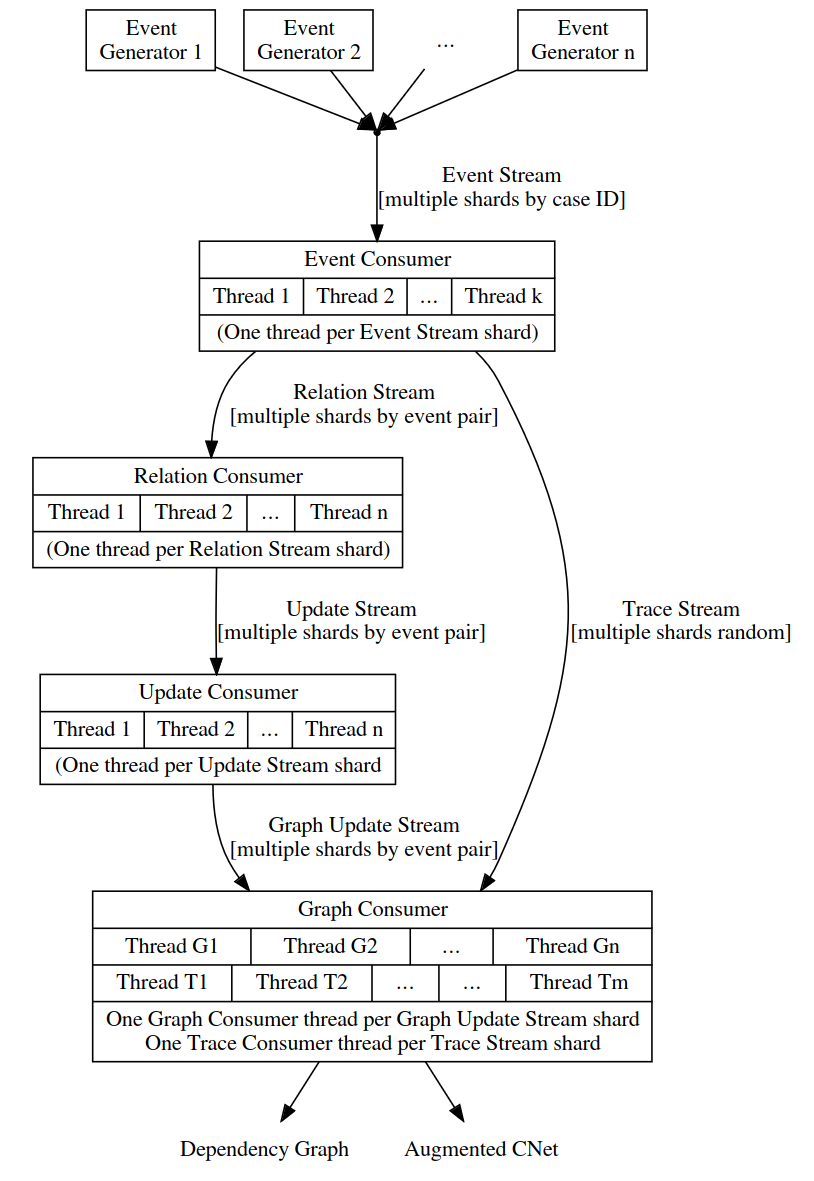
\includegraphics[width=.6\textwidth]{screen3.png} \\

\scriptsize Source: Evermann, Rehse, Fettke (2016)\normalsize
\caption[FHM on AWS Kinesis -- system architecture]{Flexible Heuristics Miner implemented on AWS Kinesis, system architecture}
\label{fig:fhmkinesis}
\end{figure}

Running on 5 compute nodes, the system is able to process over 5 million events per minute, or over 150,000 complete process traces per minute and continuously updates the discovered process model. Figure~\ref{fig:fhmkinesisperformance} shows the data throughput for each of the data streams in the system during a 3-hour period; the vertical axis is in millions of records processed.

\begin{figure}
\centering

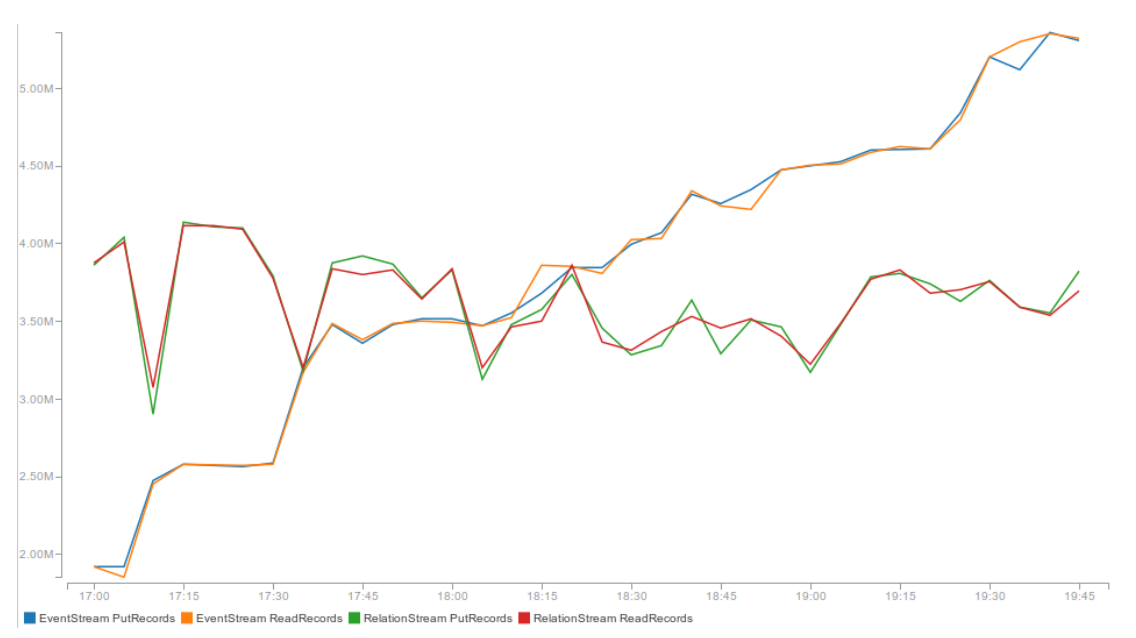
\includegraphics[width=.75\textwidth]{screen4.png} \\

\scriptsize Source: Evermann, Rehse, Fettke (2016) \normalsize
\caption[FHM on AWS Kinesis -- data throughput]{Flexible Heuristics Miner implemented on AWS Kinesis, data throughput}
\label{fig:fhmkinesisperformance}
\end{figure}

\FloatBarrier
\section{Spark Streaming}

Apache Spark Streaming enables scalable, high-throughput, fault-tolerant stream processing of live data streams. It can ingest data from various sources like Kafka, Flume, Kinesis, or network sockets, and process it using algorithms expressed with high-level functions like map, reduce, join, and window. Spark Streaming can provide output to a number of destinations, such as distributed file systems, databases, and visual dashboards (Figure~\ref{fig:sparkstreaming1}).

\begin{figure}
\centering

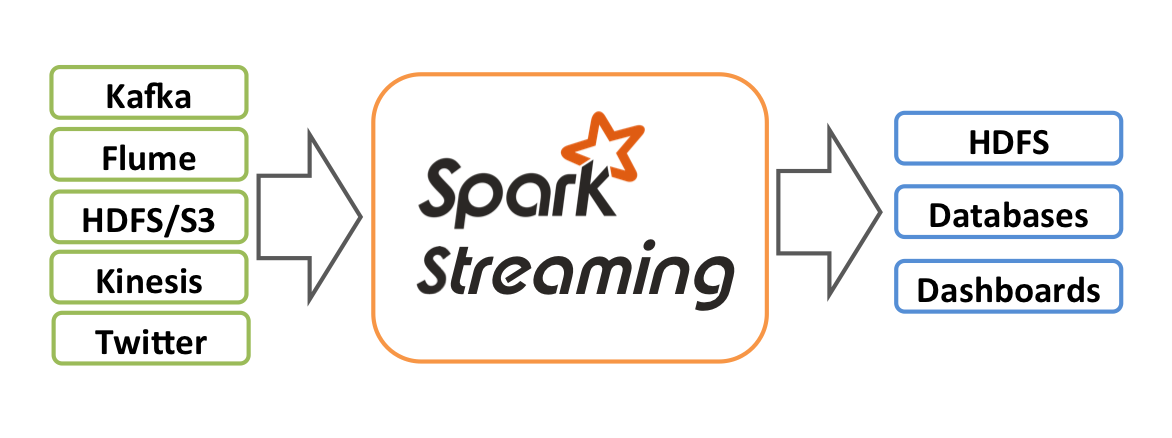
\includegraphics[width=.75\textwidth]{streaming-arch.png} \\
\scriptsize\url{https://spark.apache.org/docs/latest/img/streaming-arch.png}\normalsize \\

\caption{Spark Streaming input sources and output destimations}
\label{fig:sparkstreaming1}
\end{figure}

Spark Streaming processes live streams of data in small batches, known as \emph{micro-batches}, containing one or a few data records. This allows the framework to achieve high throughput and low latency. These micro-batches are created at user-defined intervals and processed by the Spark engine to generate the final stream of results in batches (Figure~\ref{fig:sparkstreaming2}).

\begin{figure}
\centering

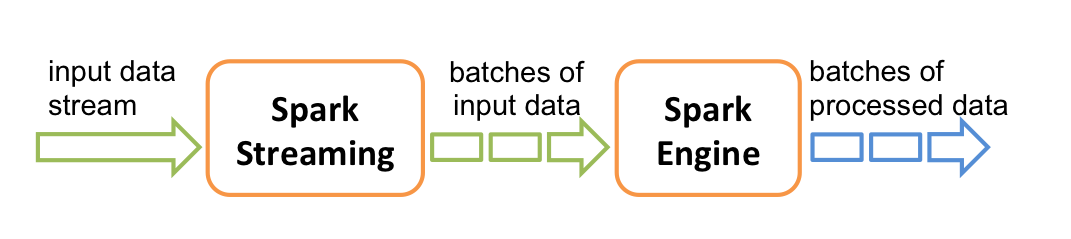
\includegraphics[width=.75\textwidth]{streaming-flow.png}  \\

\scriptsize\url{https://spark.apache.org/docs/latest/img/streaming-flow.png}
\caption{Speark Straming batches}
\label{fig:sparkstreaming2}
\end{figure}

Spark Streaming represents data streams as unbounded tables (Figure~\ref{fig:sparkstreamtable}). With this representation Spark provides a unified programming model for both batch and stream processing, using the same Spark DataFrame operations for both modes. Spark Streaming can be combined with other big data tools supported by Spark, such as Spark SQL, MLLib for machine learning, and GraphX for graph processing. This integration allows for seamless data processing pipelines that include streaming data, batch data, and interactive queries.

\begin{figure}
\centering

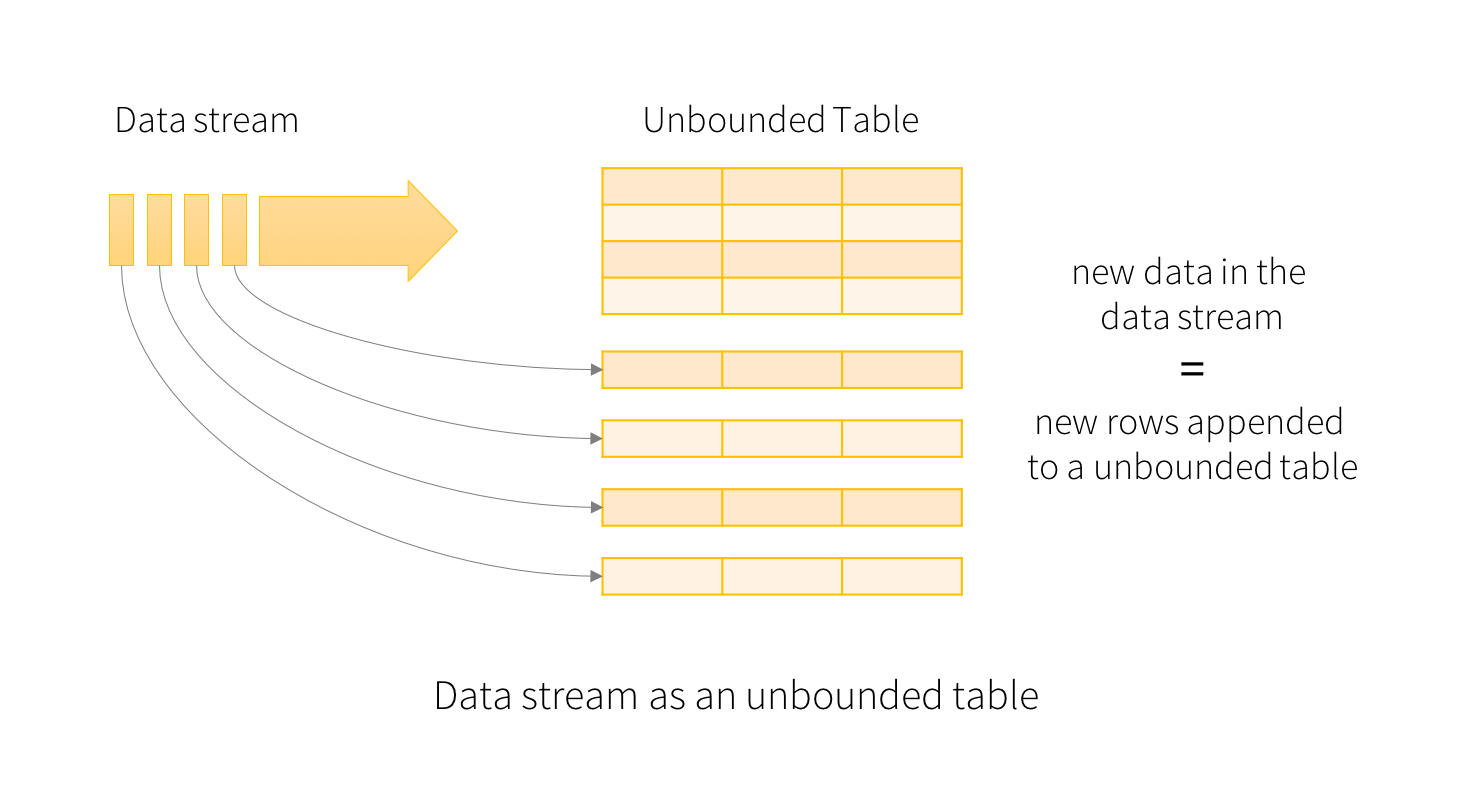
\includegraphics[width=\textwidth]{stream-as-a-table.png} \\

\scriptsize\url{https://spark.apache.org/docs/latest/img/structured-streaming-stream-as-a-table.png}
\caption{Spark data stream as an unbounded table}
\label{fig:sparkstreamtable}
\end{figure}

Spark Streaming supports stateful computations, allowing it to \emph{maintain state} across different batches of data. This is crucial for applications that require tracking session information or aggregating data over time. Spark Streaming also provides capabilities for \emph{windowed computations}, where data transformations are applied over a sliding window of data. This is essential for tasks that need to group and aggregate data over specific time frames.

Apache Spark Streaming provides various options for controlling the timing of streaming data processing through its trigger modes, and different ways of managing output data via output modes. \emph{Triggers} in Apache Spark Streaming determine how often the streaming data should be processed. There are several types of triggers:

\begin{itemize}
\item \emph{Micro-batch}: The next micro-batch is processed as soon as the previous micro-batch is completed. This mode aims to achieve the highest possible throughput by keeping the system continuously busy.

\item \emph{Fixed time interval}: This trigger processes micro-batches at user-specified fixed intervals, such as every 5 seconds. This is useful for scenarios where data should be processed at regular, predictable intervals.

\item \emph{Once}: A one-time trigger processes a single batch in response to an event or as a one-off computation. This can be useful for testing or for updating results at irregular intervals.

\item \emph{Continuous}: In continuous processing mode, Spark processes records immediately as they arrive, which significantly lowers the end-to-end processing time (latency). This mode is still experimental and may not support all the features of structured streaming.
\end{itemize}

\emph{Output modes} in Spark Streaming dictate what gets written to the output destination at the end of each trigger interval. There are several output modes to choose from:

\begin{itemize}
\item \emph{Complete Mode}: In this mode, the entire updated result table is outputted after every trigger. It is suitable for scenarios where the full snapshot of the table is needed after each processing interval.

\item \emph{Append Mode}: This mode is used when you only want to output the rows that were added to the result table since the last trigger. It is commonly used for cases where only new data is of interest (e.g., new records from a stream).

\item \emph{Update Mode}: The update mode outputs only the rows that were updated in the result table since the last trigger. It does not output the rows that have not changed, making it more efficient than complete mode if only changes are necessary.
\end{itemize}

Spark Streaming is integrated with Spark ML machine learning. It provides streaming implementations of basic machine learning models (linear regression, logistic regression, k-means clustering) that can be trained on continuous data streams. Spark Streaming also offers the ability to predict from data stream for models that were trained off-line, for models created by Spark ML.

\subsubsection*{Example}

To illustrate Spark Streaming, the following PySpark example implements a real-time word count system that ingests data from a network connection (''socket'')\footnote{Source: \url{https://spark.apache.org}}.

The first Python code block imports all necessary functions:

\begin{samepage}
\begin{pythoncode}
from pyspark.sql.functions import explode, split, col, desc, \
    window, current_timestamp
\end{pythoncode}
\end{samepage}

The next code block creates a stream reader to read from a network socket on the local machine on port number 9999. The result, \texttt{lines}, is a Spark DStream object representing the input data stream. Note that the stream reader opens a \emph{client} socket, i.e. the socket must already have been opened for writing by the data producer, otherwise the \texttt{load()} action will fail.

\begin{samepage}
\begin{pythoncode}
lines = spark.readStream \
             .format('socket') \
             .option('host', 'localhost') \
             .option('port', 9999) \
             .load()
\end{pythoncode}
\end{samepage}

Next, processing of individual lines is done, using the same functions as in the earlier Spark DataFrame examples. In the following block of Python code \texttt{words} is another DStream that is connected to the \texttt{lines} DStream, as illustrated in Figure~\ref{fig:sparkwordcount}.

\begin{samepage}
\begin{pythoncode}
words = lines.select(explode(split(col('value'),'\\s')).alias('word'))
\end{pythoncode}
\end{samepage}

\begin{figure}
\centering

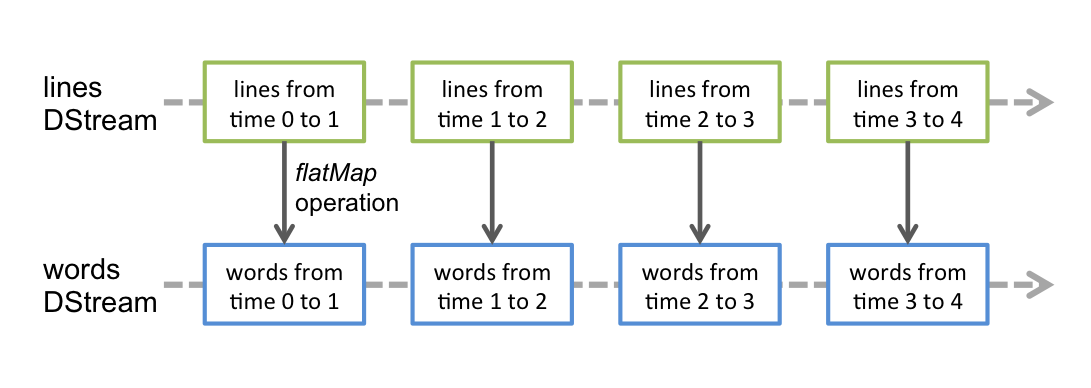
\includegraphics[width=\textwidth]{streaming-dstream-ops.png}
\scriptsize\url{https://spark.apache.org/docs/latest/img/streaming-dstream-ops.png}\normalsize
\caption{Spark Streaming line and word DStreams}
\label{fig:sparkwordcount}
\end{figure}

Individual words are then processed, again, in the same way as in the earlier Spark DataFrame example. The following Python code block creates \texttt{counts} as another Dstream, connected to the \texttt{words} DStream.

\begin{samepage}
\begin{pythoncode}
counts = words.groupBy('word') \
              .count() \
              .sort(desc('count'))
\end{pythoncode}
\end{samepage}

Finally, an output writer is defined with a ''complete'' output mode that writes the complete result after each micro-batch, and a 5 second timer interval trigger on processing -- Spark Streaming will read and process a micro-batch every 5 seconds. The checkpoint location is where Spark Streaming stores information about the status of the data streams so it can recover in case processing is interrupted. This ensures fault tolerance, and allows Spark Streaming to guarantee that every record is processed and every record is processed only once. Figure~\ref{fig:streamingexample} illustrates the complete example.

\begin{samepage}
\begin{pythoncode}
writer = counts.writeStream \
           .format('console') \
           .outputMode('complete') \
           .trigger(processingTime='5 second') \
           .option('checkpointLocation', \
               'hdfs://localhost:9000/user/busi4720/')
\end{pythoncode}
\end{samepage}

\begin{figure}
\centering

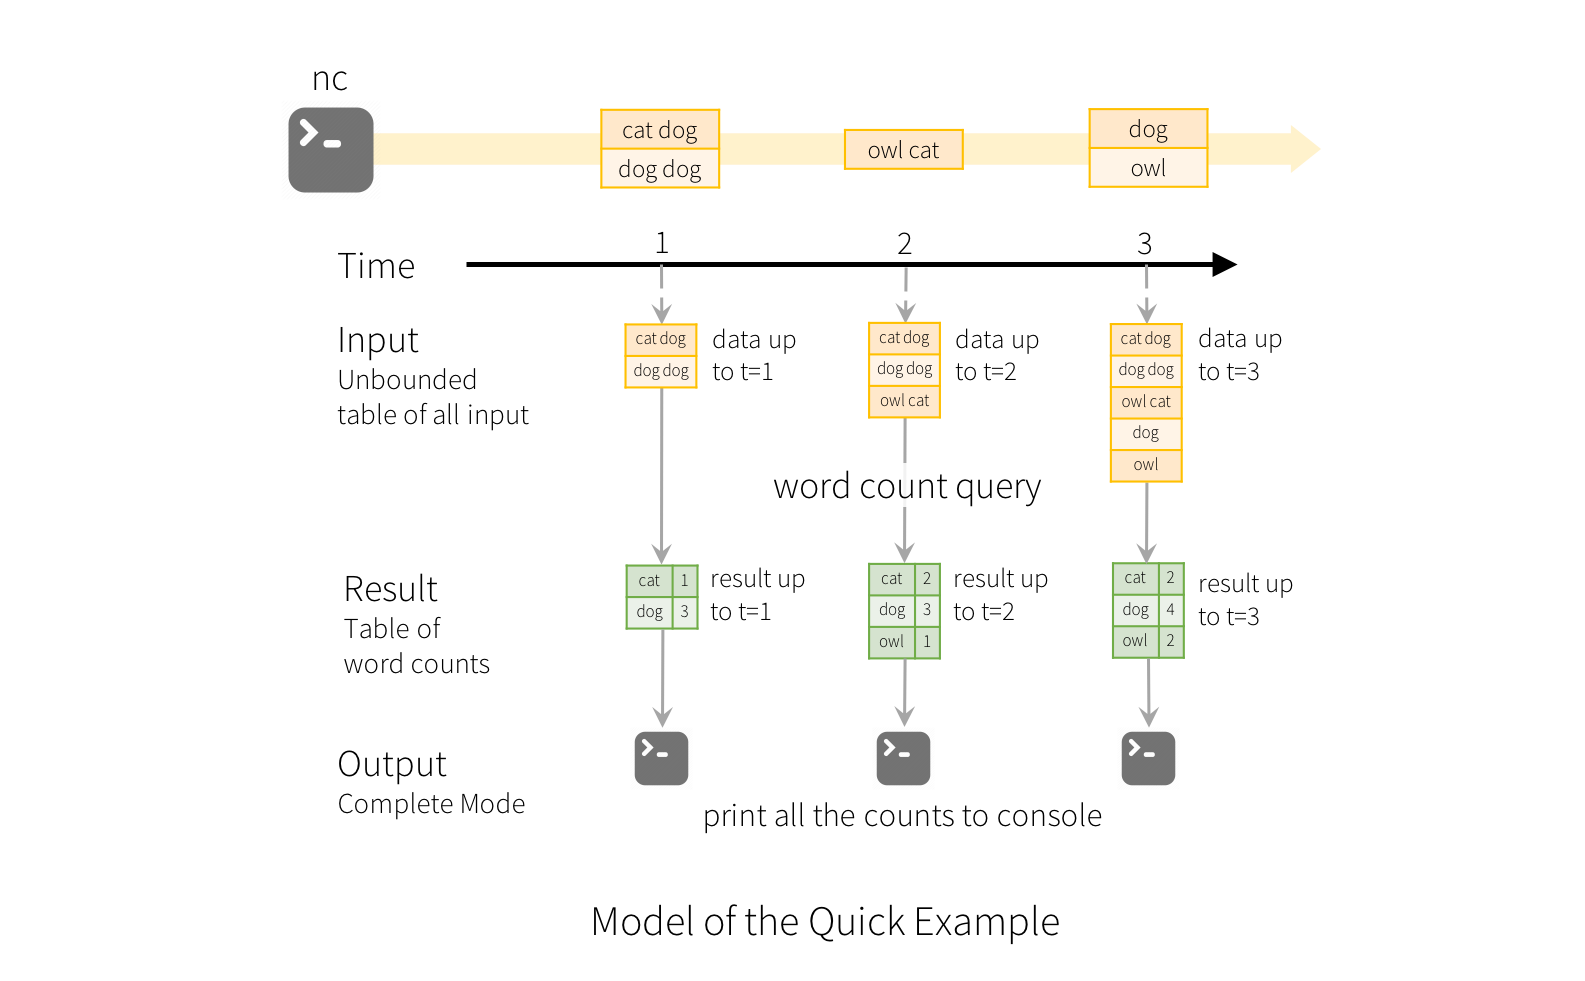
\includegraphics[width=\textwidth]{structured-streaming-example-model.png} \\

\scriptsize\url{https://spark.apache.org/docs/latest/img/structured-streaming-example-model.png}
\caption{Spark Streaming complete word count example}
\label{fig:streamingexample}
\end{figure}

To see this Spark Streaming application in operation, use a Bash command shell to open a network socket using the \texttt{nc} command:

\begin{bashcode}
nc -kl 9999
\end{bashcode}

Then, start the stream data processing by starting the writer. This returns a streaming query object that provides progress information. The ''\texttt{start()}'' method is a non-blocking operation so that stream processing will occur in the background.

\begin{pythoncode}
streamingQuery = writer.start()
\end{pythoncode}

The query object can be used to get progress information, through its \texttt{lastProgress} attribute:

\begin{pythoncode}
print(streamingQuery.lastProgress)
\end{pythoncode}

The query object also provides a \texttt{stop()} method to end the processing:

\begin{pythoncode}
streamingQuery.stop()
\end{pythoncode}

This basic example can be extended to illustrate time windowing, illustrated in the following Python code block. First, the line processing is changed to not only split lines into words, but also to record the event timestamp. That is, the \texttt{words} DStream will contain two columns, \texttt{word} and \texttt{eventTime}:

\begin{samepage}
\begin{pythoncode}
words = lines \
    .select(explode(split(col('value'),'\\s')).alias('word')) \
    .withColumn('eventTime', current_timestamp())
\end{pythoncode}
\end{samepage}

The following Python code block changes the definition of the \texttt{counts} DStream to group by words but now for one minute windows of the \texttt{eventTime} column; windows are updated every 30 second, that is, overlapping time windows. Figure~\ref{fig:streamingtimewindow} illustrates the time windowing concept.

\begin{samepage}
\begin{pythoncode}
counts = words \
    .groupBy('word', window('eventTime', '1 minute', '30 second')) \
    .count() \
    .sort(desc('count'))
\end{pythoncode}
\end{samepage}

\begin{figure}
\centering
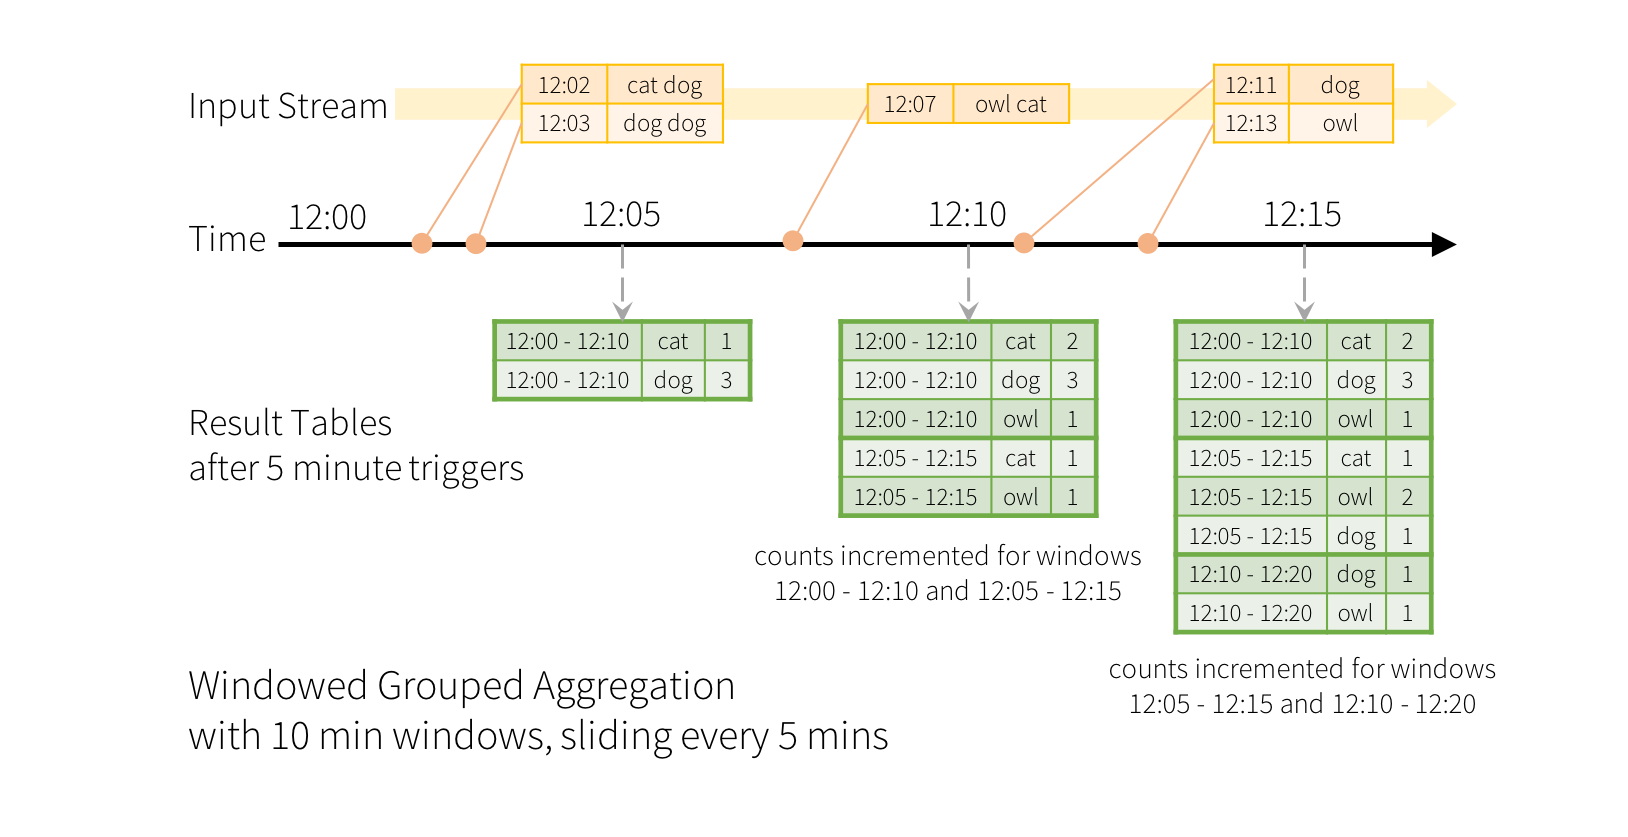
\includegraphics[width=\textwidth]{structured-streaming-window.png} \\

\scriptsize\url{https://spark.apache.org/docs/latest/img/structured-streaming-window.png}
\caption{Spark Streaming time windowing}
\label{fig:streamingtimewindow}
\end{figure}

\FloatBarrier
\section{Review Questions}
\paragraph*{Introduction}
\begin{enumerate}[nosep]
    \item Define big data analytics and discuss its significance to business practices.
    \item What are the three main ''V''s of big data? Explain how they characterize big data challenges and opportunities.
	\item The text mentions two additional Vs, veracity and value. Describe these concepts and explain their importance in the context of big data.
	\item Why is timely data processing important in scenarios involving high-velocity data? Provide an example where delay in data processing could be detrimental.
    \item What are the implications of poor data veracity? How can organizations ensure the accuracy and reliability of their data?
    \item Discuss the concept of value in big data. What steps must organizations take to transform big data into actionable insights?
	\item What are some challenges organizations face when scaling from desktop data analysis tools to industrial-scale big data analytics platforms?
\end{enumerate}
\paragraph*{Apache Hadoop}
\begin{enumerate}[nosep,resume*]
	\item Describe the primary function of Apache Hadoop and its origins.
	\item Explain the concept of 'data locality' in the context of Hadoop. Why is it beneficial to process data where it is stored?
	\item What are the three main components of Hadoop? Briefly describe the role of each component.
	\item Discuss the reliability features of Hadoop. How does Hadoop ensure data is not lost in case of a node failure?
	\item Describe the process of data replication in HDFS. Why is data replicated across different nodes, and how does this impact system performance?
	\item Explain the architecture of HDFS. What are the roles of the NameNode and DataNodes?
	\item What are the limitations of the Hadoop ecosystem, and how have new developments or additional tools addressed these challenges?
	\item Reflect on how the principles of Hadoop (for example, data locality and redundancy) apply to practical scenarios such as disaster recovery and data processing efficiency.
	\item Discuss the impact of Hadoop's 'write once, read many times' model on data analysis tasks. What types of applications are best suited for this model?
\end{enumerate}
\paragraph*{MapReduce}
\begin{enumerate}[nosep,resume*]
	\item Define the MapReduce programming model and explain its primary purpose in handling large data sets.
	\item Describe the roles of the Map and Reduce functions in a MapReduce job. What types of operations might each perform?
	\item Explain the process of data flow from input to output in a MapReduce job, including the stages of Map, Shuffle, and Reduce.
	\item Discuss how MapReduce utilizes the distributed storage provided by HDFS for both computation and storage of intermediate results.
	\item What are the limitations of the MapReduce model regarding the types of data flows it supports? Why does it struggle with iterative or cyclic data flows?
	\item Describe the roles of the Resource Manager and NodeManager in the YARN architecture. How do they interact during the execution of a MapReduce job?
	\item What happens during the shuffle phase of a MapReduce job? Explain how data is distributed and prepared for the Reduce phase.
	\item Explain the role of the Application Master in a MapReduce job executed on a YARN cluster. How does it manage job execution and resource allocation?
	\item How does the number of Reduce instances relate to the number of unique key values in the input data? What determines the number of Reduce tasks in a job?
	\item What is the purpose of the Map function in the MapReduce model? Provide an example of a simple Map function.
	\item Explain the concept of key-value pairs in the context of MapReduce. How are these used throughout the MapReduce process?
	\item Discuss how the Reduce function aggregates the outputs from the Map function. Provide an example where this aggregation is critical to the outcome of the MapReduce job.
	\item Why might intermediate data in a MapReduce job be larger than the input data? What challenges does this present?
\end{enumerate}
\paragraph*{Apache Pig}
\begin{enumerate}[nosep,resume*]
	\item What is Apache Pig?
	\item Explain the main features of Pig Latin and how it simplifies writing data analysis programs compared to MapReduce.
	\item What are some of the core operations in Pig Latin? Provide examples of how two of these operations can be used in data processing.
	\item Compare and contrast the procedural nature of Pig Latin with the declarative nature of SQL. What are the implications of each approach for data analysis?
\end{enumerate}
\paragraph*{Apache Hive}
\begin{enumerate}[nosep,resume*]
	\item What is Apache Hive and what need does it fill within the Hadoop ecosystem?
	\item What are the benefits of Hive transforming HiveQL queries into MapReduce jobs?
	\item How do Hive and Pig differ in terms of their approach to handling data on Hadoop? Consider aspects such as ease of use, flexibility, and the type of abstraction they provide.
\end{enumerate}
\paragraph*{Apache Spark}
\begin{enumerate}[nosep,resume*]
    \item What is Apache Spark and why is it considered a unified analytics system?
	\item What is the primary reason for Apache Spark's fast adoption in the industry compared to Hadoop's MapReduce?
    \item Explain the concept of in-memory cluster computing in Spark. How does this improve processing speed compared to disk-based systems like MapReduce?
    \item How does Spark integrate with existing Hadoop clusters and why is this beneficial for users already using Hadoop?
    \item Describe the various types of workloads that Spark's unified engine can handle. How does this versatility affect system management and efficiency?
    \item What are Resilient Distributed Datasets (RDDs)? Discuss their importance in Spark's architecture, including how they handle failures.
	\item Describe the concept of data lineage in Spark's architecture. How does it assist in the re-computation of RDDs if part of the data or process is lost?
    \item Explain the role of Spark SQL within the Apache Spark ecosystem. How does it integrate traditional SQL database functionality with big data processing?
    \item Discuss the execution principles of Apache Spark, focusing on transformations and actions. What does lazy execution mean and why is it beneficial?
    \item How does Apache Spark manage large-scale data processing across a cluster? Explain the roles of the driver program, cluster manager, and worker nodes.
	\item What is a schema in the context of Apache Spark, and what purposes does it serve?
	\item Describe a scenario where using SQL to operate on a DataFrame could be more advantageous than using DataFrame API methods directly.
\end{enumerate}
\paragraph*{Apache Spark Machine Learning}
\begin{enumerate}[nosep,resume*]
    \item Explain the concept of a machine learning pipeline in Spark ML. How does it enhance the workflow of machine learning models?
    \item What is a \emph{Transformer} in Spark ML, and what role does it play in a machine learning pipeline? Provide examples.
    \item Describe what an \emph{Estimator} is and its function within the Spark ML framework. Include examples of common estimators.
	\item How does Spark ML leverage the concept of lazy execution in its machine learning pipelines?
    \item Detail how a fitted machine learning pipeline acts as a transformer. What does this imply for new input data?
\end{enumerate}
\paragraph*{Apache Spark Streaming}
\begin{enumerate}[nosep,resume*]
	\item Define stream analytics and contrast it with batch processing. What are the key characteristics that differentiate the two?
	\item Explain why stream analytics is essential for data with high volume and velocity. Provide examples of scenarios where stream analytics is preferable.
	\item Explain the importance of real-time decision-making in stream analytics. How does this impact the design of stream processing systems?
	\item Describe the unified programming model of Spark Streaming. How does it enable seamless transition between batch and stream processing?
	\item Explain the concept of micro-batching in Spark Streaming. How does it contribute to achieving high throughput and low latency?
	\item Discuss the different trigger modes available in Spark Streaming. What are the use cases for each mode?
	\item What are the output modes available in Spark Streaming and how do they differ? Provide scenarios in which each would be used.
	\item Analyze the benefits and limitations of using continuous processing mode in Spark Streaming. What types of applications benefit most from this mode?
\end{enumerate}
